\documentclass[a4paper]{article}

\usepackage[english]{babel}
\usepackage[utf8]{inputenc}
\usepackage{amsmath}
\usepackage{float}
\usepackage{graphicx}
\usepackage{subcaption}
\usepackage[colorinlistoftodos]{todonotes}
\usepackage{hyperref}
\usepackage{lineno}
\usepackage{setspace}
\usepackage{soul}
\usepackage{multirow}
\usepackage[affil-it]{authblk}
\usepackage{verbatim}
\usepackage[bottom]{footmisc}
\usepackage[left=0.6in,right=0.6in,top=1in,bottom=1in]{geometry}
\usepackage[margin=0.6in]{caption}
\usepackage{multicol}
\usepackage{lineno}
\linenumbers
\linespread{1.1}

\usepackage{listings}
\usepackage{xcolor}
\lstset { %
    language=C++,
    backgroundcolor=\color{black!5}, % set backgroundcolor
    basicstyle=\footnotesize,% basic font setting
}

\title{Measurement of $\nu_e$ interactions at low energy with the MicroBooNE Experiment}

\author[1]{Sophie Berkman}
\author[1]{David Caratelli}
\author[2]{Ivan Caro Terrazas}
\author[1]{Giuseppe Cerati}
\author[3]{Nicolo Foppiani}
\author[1]{Elena Gramellini}
\author[3]{Roxanne Guenette}
\author[2]{Ryan LaZur}
\author[2]{Michael Mooney}
\author[3]{Sebasten Prince}
\author[3,4]{Roberto Soleti}
\author[3,4]{Wouter Van De Ponteele}
\author[1]{Maya Wospakrik}
\affil[1]{Fermi National Accelerator Laboratory}
\affil[2]{Colorado State University}
\affil[3]{Harvard University}
\affil[4]{University of Oxford}
%\date{\today}	


\begin{document}

\maketitle

\abstract{We present an analysis which measures $\nu_e$ interactions from the Booster Neutrino Beamline with the MicroBooNE Experiment with the goal of addressing the nature of anomalous low-energy events with EM activity in the final state recorded by the MiniBooNE experiment. In this document we report the reconstruction and event selections performed, the evaluation of systematics associated to detector, flux, and neutrino-interaction modeling, and the expected sensitivity to the MB-$\nu_e$ LEE model utilizing the available BNB dataset of 10.1$\times 10^{20}$ POT. }

\tableofcontents

\newpage

%\begin{multicols}{1}
\section{Introduction to the $\nu_e$ analysis}
\begin{comment}
\par The analysis presented in this note consists in a measurement of $\nu_e$ interactions from the BNB with MicroBooNE in the low-energy ($\lt 800$ MeV) regime aimed at addressing the electron or photon-like nature of MiniBooNE's recorded excess of events with EM activity in the final state. 
This analysis focuses on being able to measure low-energy $\nu_e$ interactions. The reason for this is to have sensitivity to a potential signature of anomalous $\nu_e$ events which comprise MiniBooNE's Low Energy Excess (LEE). This excess was recorded below 800 MeV in reconstructed visible energy (most hadronic activity, especially protons, because below Cherenkov threshold). 
\end{comment}
\subsection{$\nu_e$ Selection Philosophy}
\par Several proposals have been made to explain the nature of the MiniBooNE LEE anomaly, and it is fair to say that a large amount of uncertainty remains in the community regarding what may have generated such anomalous EM events. In order to be best prepared to address the question of whether potential new physics can be seen in the $\nu_e$ channel in the BNB at low energy, this analysis aims to perform an inclusive multi-channel measurement of $\nu_e$ interactions without relying on neutrino-interaction model dependent kinematics. 
\par \textbf{multi-channel approach}  To achieve this, we perform three $\nu_e$ selections, each aimed at leveraging particular strengths, and designed with cuts tailored to exploit as much information in a given channel topology as possible. The analysis is comprised of a $\nu_e$ inclusive, a 1$e$N$p$, and a 1$e$0$p$ selection. A schematic summarizing the strengths and features of each selection is shown in figure~\ref{fig:nueselections}. The 1$e$N$p$ and 1$e$0$p$ selections are orthogonal and share a common pre-selection, which splits at the stage in which presence of a final state proton in the event is determined. The inclusive $\nu_e$ selection currently is developed independently of the 1$e$N$p$ selection and therefore its selected events are not independent.

\begin{figure}[ht]
\begin{center}
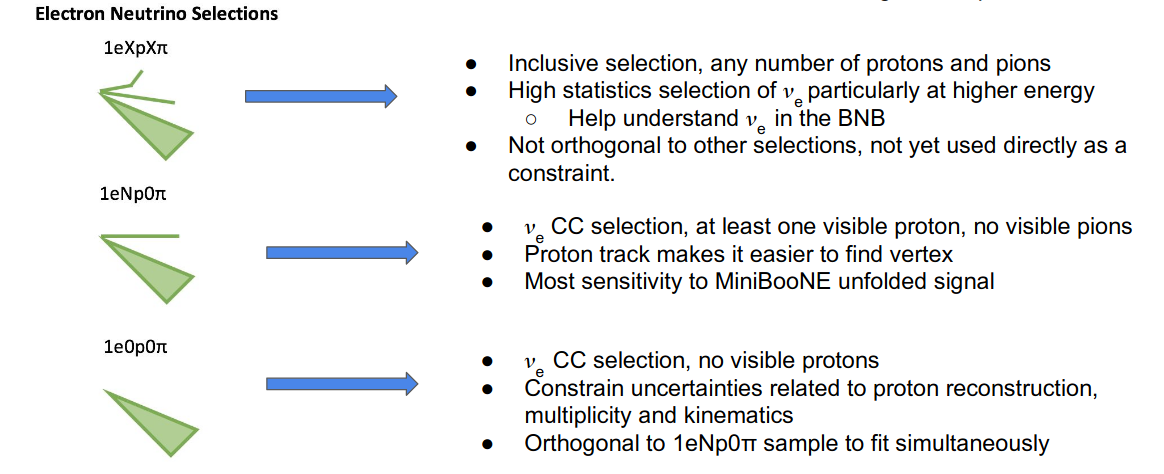
\includegraphics[width=0.85\textwidth]{introduction/nueselections.png}
\caption{\label{fig:nueselections}Schematic of the three $\nu_e$ selection in this analysis, outlining the goals and strengths of each. In this work, the threshold for a visible proton at truth-level proton is 40 MeV of KE. $N$ refers to one or more and $X$ to any number of final state particles of a given category.}
\end{center}
\end{figure}

\par \textbf{agnostic selection} In devising the selections presented above, we have deliberately chosen to not rely on cuts that make use of kinematic features of low-energy $\nu_e$ events. This allows the analysis to be agnostic to possible sources of new physics, and limits model dependence associated with assumptions on intrinsic $\nu_e$ interaction kinematics. Furthermore, an agnostic selection strategy allows to explore the kinematics of $\nu_e$ candidate events after their selection, for a full investigation of the origin of a potential anomaly.




\subsection{Signal Model}
\par In order to benchmark the performance of the analysis it is valuable to have a signal model which can be used to assess the sensitivity to a possible model addressing the MiniBooNE LEE result. This section describes the choice of model used for this purpose. It is important to stress that the signal model used serves the purpose of benchmarking the analysis' sensitivity, but the ultimate goal of the analysis remains to measure the rate of $\nu_e$ interactions in the BNB and report whether the observation is consistent or not with MicroBooNE's prediction. Answering whether MicroBooNE's observation is consistent or not with the MiniBooNE LEE anomaly is beyond the scope of this work, and something not achievable without significant work for both MiniBooNE and MicroBooNE.
\par To test this analysis' sensitivity to MiniBooNE's LEE, a model which can explain it as an excess of $\nu_e$ interactions must be produced, and used to generate simulated events in MicroBooNE. Many such models can be devised, each relying on a given (new) physics production mechanism and set of assumptions on detector response. The primary sensitivity quoted by this analysis will focus on the MiniBooNE-unfolded LEE model, referred to as \textbf{MB-$\nu_e$ LEE} model in this document. In this model, excess LEE events are assumed to be due to $\nu_e$ interactions with a value of true energy obtained by unfolding LEE events with a reconstructed energy obtained through the CCQE formula by relying on MiniBooNE's energy smearing matrix. The resulting true neutrino energy distribution is shown in figure~\ref{fig:minibooneunfolded}. There are several limitations to this model worth observing, some technical, others conceptual. On a technical level, the model is composed of a binned event distribution, rather then a parametrized or analytic prediction of the expected $\nu_e$ spectrum. Additionally, no events below 200 MeV of true energy exist in this model. These two factors lead to a granular and truncated model prediction.
\begin{figure}[ht]
\begin{center}
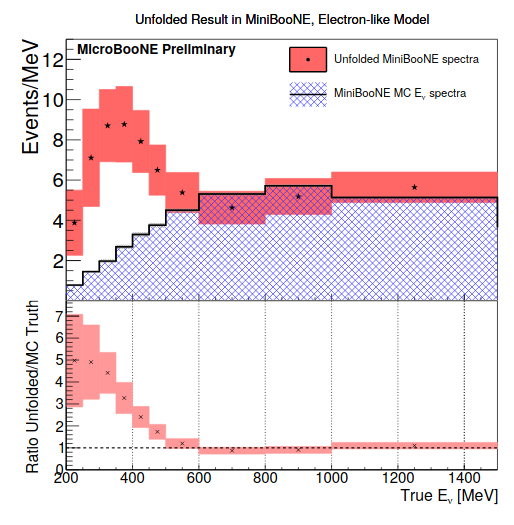
\includegraphics[width=0.45\textwidth]{introduction/unfoldedminiboone.png}
\caption{\label{fig:minibooneunfolded}MB-$\nu_e$ LEE signal model extracted from MiniBooNE's results.}
\end{center}
\end{figure}
Conceptual issues can be raised in association with the various assumptions made to generate the model. These include the strong reliance on MiniBooNE's simulation in order to unfold reconstructed to true neutrino energy, and the choice of such an unfolding procedure (performed as a function of $E_{\rm CCQE}$ rather then EM energy and $\theta$, for example).
\par Ultimately many signal models can be produced to test an analysis' sensitivity, each with its own set of important assumptions and caveats. While reporting sensitivities for the MB-$\nu_e$ LEE model is useful, it is not exhaustive in being able to address MicroBooNE's ability to address MiniBooNE's anomaly. It is especially important to note that this model strongly favors the interpretation of MiniBooNE events as originating from very low energies (200-400 MeV) for which achieving high sensitivity may come at the cost of omitting a robust analysis at higher energies. This is something the analysis tries to avoid by developing an inclusive and kinematically unbiased analysis workflow. At the same time, we explore additional models for sensitivity calculations, most notably a 3+1 sterile-neutrino oscillation model. This is discussed in more detail in section~\ref{sec:sensitivity}.
\subsection{Goals of the $\nu_{\mu}$ Selection}
\par For the purpose of this analysis, measurements of $\nu_{\mu}$ interactions are aimed at reducing modeling uncertainties for intrinsic $\nu_e$ and background categories, with the goal of reducing systematic uncertainties in order to be able to claim the observation of new physics were a measurement of $\nu_e$ interactions differ significantly from the expected intrinsic rate. This section describes why such a data-driven constraint is needed and what are the choices which motivate the approach taken in this analysis.
\par Event reconstruction and $\nu_e$ identification are only one of the challenges in this analysis. In order to move from being able to produce a high-quality $\nu_e$ measurement to being able to make statements on whether the observed $\nu_e$ rate indicates a presence of new physics, a well understood prediction of the intrinsic $\nu_e$ expected is needed. Uncertainties in the expected $\nu_e$ rate are associated to reconstruction efficiencies (detector effects) as well as modeling uncertainties in both the $\nu_e$ flux prediction and neutrino-argon cross-section models. Here we focus on describing the strategy employed to deal with these modeling uncertainties. Modeling uncertainties in the expected rate of $\nu_e$ interaction are large, and can limit the ability to associated a $\nu_e$ measurement with potential new physics if not constrained through additional measurements. Flux uncertainties for $\nu_e$ are $\mathcal{O}$(10\%) above 800 MeV and grow to 40\% at 200 MeV. Cross-section uncertainties are also large, a consequence of a lack of measurements of $\nu$-Ar cross-sections, particularly at low energy, and the complex modeling of neutrino interactions on a heavy target such as argon. In the few-hundred MeV energy range modeling uncertainties are such that MicroBooNE's cross-section predictions are of the order 100\%.
\par To reduce modeling uncertainties on the expected rate of $\nu_e$ interactions, additional measurements capable of reducing systematic uncertainties at low energies are required. This can be achieved by performing measurements of $\nu_{\mu}$ interactions subject to the same uncertainties. In order to constrain flux uncertainties, we rely on the fact that $\nu_e$ and $\nu_{\mu}$ intrinsic to the beam are produced by the decay of the same parent $\pi$ and $K$ flux. Similarly for uncertainties on neutrino interaction modeling, we rely on the common charged-current interaction mode $\nu_{l} + Ar \rightarrow l + X$ for both $\nu_{\mu}$ and $\nu_e$ interactions to constrain interaction uncertainties. 
\par The complexity of $\nu$-Ar interactions and of hadronic interactions in the beamline mean that many different handles and measurements of $\nu_{\mu}$ interactions can play a role in constraining different uncertainties. As examples, measurement of CC and NC $\pi^0$ production constrain resonant interactions and thus $\pi^0$ backgrounds to the $\nu_e$ selection, and measurements of high-energy $\nu_{\mu}$ interactions can help constrain the kaon flux in the beam, which contributes substantially to the production of intrinsic $\nu_e$s. Likewise, measurements of low-energy $\nu_{\mu}$s can help constrain poorly understood $\nu$-Ar interaction models in the few-hundred MeV energy regime, a critical requirement for this analysis. The neutrino identification work developed for this analysis, referred to as \emph{SliceID} and described in section~\ref{sec:sliceID}, is a highly efficient and topology agnostic selection that enables a vast program of $\nu_{\mu}$ measurements, allowing for flexibility in selecting topologies that may have the strongest constraining power and thus most benefit the $\nu_e$ analysis. At the current time, as described in the remainder of this section and in section~\ref{sec:systematics}, the emphasis is on the measurement of low-energy $\nu_{\mu}$ interactions with the goal of constraining the large uncertainties in low-energy $\nu_e$ events which otherwise limit the analysis.
\par Figure~\ref{fig:numuconstraint:flux} shows the flux correlation for $\nu_{\mu}$ (bottom left) and $\nu_e$ (top right) interactions. Red (blue) areas show large (anti-)correlation. The top-left or bottom-right quadrants show the strength of correlations between the two flavors. For $\nu_e$ energies below 1 GeV, correlations are strongest with $\nu_{\mu}$ interactions at low energy. Figure~\ref{fig:numuconstraint:xsec} shows different cross-section curves for $\nu_{\mu}$ and $\nu_e$ interactions. The dashed and solid curves represent the CCQE cross-section used in MCC8 vs. MCC9 respectively. Below 400 MeV, the difference in event rates for different models is larger then 100\%. The large differences between these curves, particularly at low energy, indicate the strong need to constrain cross-section uncertainties with MicroBooNE's own data. 
\begin{figure}[ht] 
\begin{center}
    \begin{subfigure}[b]{0.52\textwidth}
    \centering
    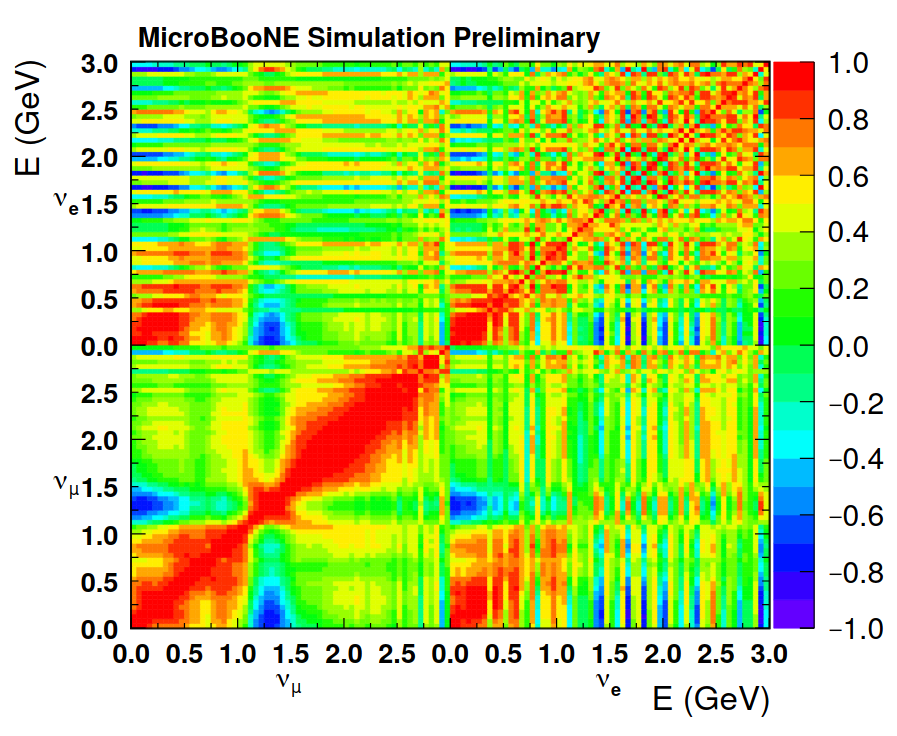
\includegraphics[width=1.00\textwidth]{introduction/fluxcorrelation.png}
    \caption{\label{fig:numuconstraint:flux}$\nu_{\mu}$-$\nu_e$flux correlation matrix}
    \end{subfigure}
    \begin{subfigure}[b]{0.4\textwidth}
    \centering
    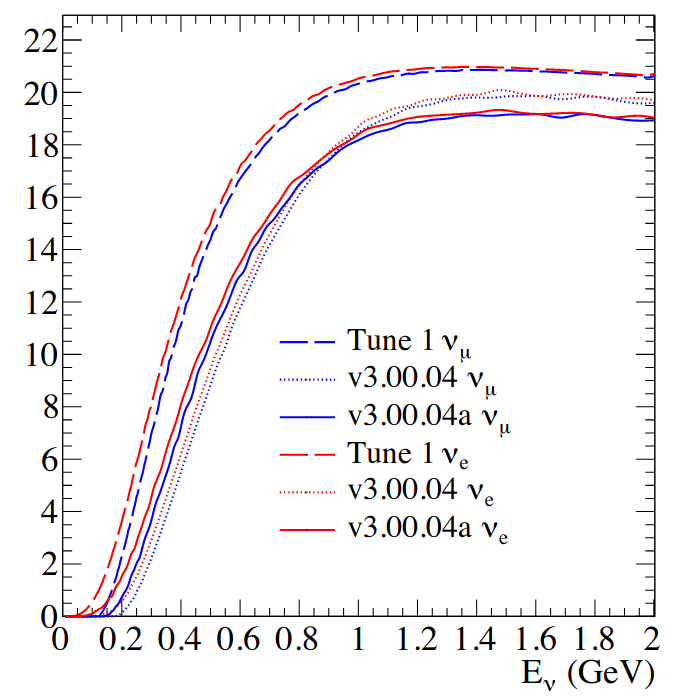
\includegraphics[width=1.00\textwidth]{introduction/xsec_mcc8_mcc9.png}
    \caption{\label{fig:numuconstraint:xsec}different xsec models for CC interactions.}
    \end{subfigure}
\caption{\label{fig:numuconstraint}}
\end{center}
\end{figure}

\subsection{Systematics}


\subsection{Sensitivity Calculation}


\newpage

\section{Overview of Neutrino Identification: Pandora SliceID}
%\subsection{Event Slicing and Cosmic Removal in Pandora}

The work presented in this note relies on the Pandora approach for event reconstruction~\cite{bib:pandoraub}. The scope of Pandora is to do the low-level pattern-recognition step of the reconstruction, i.e. group hits into clusters, clusters into particles and particles into hierarchies. This section describes how Pandora's pattern-recognition output is combined with scintillation light information to isolate possible candidate neutrino interactions in MicroBooNE events, a process illustrates in the three images of figure~\ref{fig:sliceid}. 

\begin{figure}[ht] 
\begin{center}
    \begin{subfigure}[b]{0.7\textwidth}
    \centering
    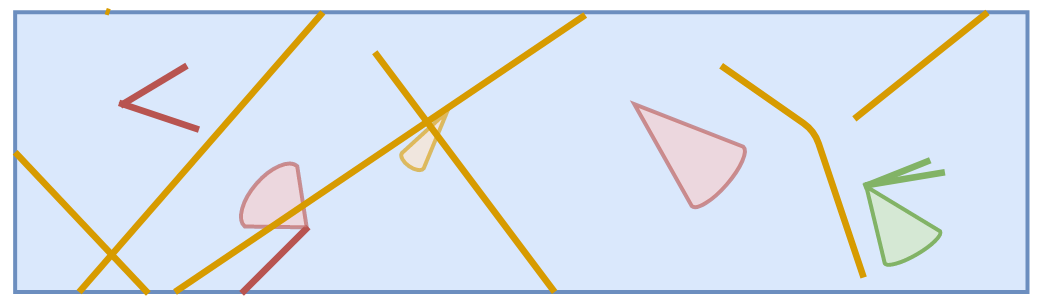
\includegraphics[width=1.00\textwidth]{NuId-Ch2/Images/slice00.png}
    \caption{\label{fig:slcieid:00} Typical event with multiple interactions isolated by Pandora in \emph{slices}.}
    \end{subfigure}
    \begin{subfigure}[b]{0.7\textwidth}
    \centering
    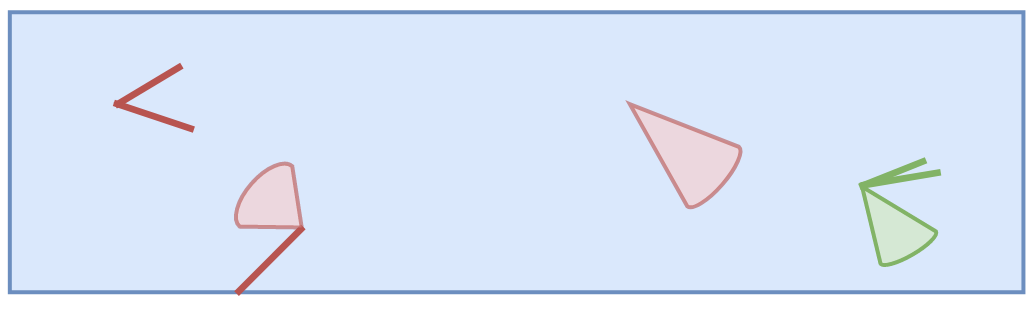
\includegraphics[width=1.00\textwidth]{NuId-Ch2/Images/slice01.png}
    \caption{\label{fig:slcieid:01} Event after the removal of \emph{obvious cosmics} tagged geometrically by Pandora.}
    \end{subfigure}
    \begin{subfigure}[b]{0.7\textwidth}
    \centering
    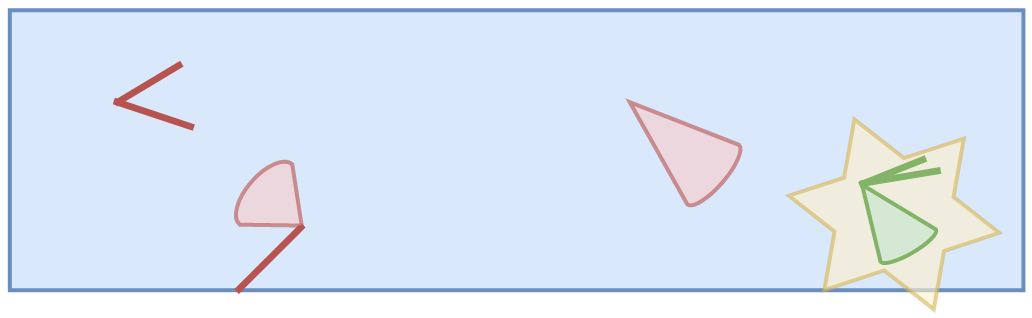
\includegraphics[width=1.00\textwidth]{NuId-Ch2/Images/slice02.png}
    \caption{\label{fig:slcieid:01} Implementation of the \texttt{SiceID} tool to isolate possible candidate $\nu$ interactions.}
    \end{subfigure}
\caption{\label{fig:sliceid} Succession of steps in cosmic removal performed using Pandora's topological pattern recognition combined with scintillation light information through the \texttt{SliceID} tool.}
\end{center}
\end{figure}

\subsection{Slicing \textcolor{green}{Wouter ... P.R. Elena}}
The creation of a ``slice" is the first step of the Pandora processing. A slice \textcolor{blue}{is a collection of distinct reconstructed particles which belong to the same interaction (such as a cosmic muon and its Michel electron, or the muon and proton in a 1$\mu$1$p$ neutrino interaction) \st{is a combination of hits on the three different planes which are topological distinct:  it is assumed that different slices correspond to a distinct group of activity in the TPC}}. To produce slices, the Pandora Cosmic Pattern Recognition is first run over all hits, aiming to construct muon tracks and associated $\delta$-rays and Michel electrons under the cosmic hypothesis (fig.~\ref{fig:sliceid:00}). At this stage, obvious cosmic activity (through-going or out-of-time muons) is tagged using geometric information. The obvious cosmic tagged hits are discarded (fig.~\ref{fig:sliceid:01}); the filtered hit collection is used as input to the Pandora Consolidated Pattern Recognition which reconstruct slices under the neutrino hypothesis. Each slice is now reconstructed both under the cosmic hypothesis and the neutrino hypothesis. A typical event contains approximately 5 slices. 

\subsubsection{Clustering and Vertex Finding \textcolor{green}{Wouter}} 
Pandora computes the 2D clustering on the hits in each slice and in each plane separately. Then, a number of 3D candidate vertices is created by finding positions that project down on to the ends of the available 2D clusters. All of the possible candidates are fed into the support vector machine (SVM) vertex selection, and the most appropriate one is chosen. This 3D vertex is used to split any existing clusters that straddle the vertex. Then, the cluster matching algorithms are run, where the clusters are compared between views and modified to improve the matching.

\subsection{SliceID : Cosmic Removal through topology and scintillation-light \textcolor{green}{Wouter}}
\label{sec:sliceID:SliceID}
\par After the Pandora pattern-recognition algorithm suite has isolated individual interactions into reconstructed \emph{slices} and removed those that are either through-going or out-of-time, the remaining task is to identify which (if any) slice is associated to a neutrino interaction. This is done by relying on scintillation light information to reject slices incompatible with light recorded in-time with the beam. Additionally, topological cuts aimed at rejecting stopping-muon events which enter the TPC are used. The SliceID is at the core of all neutrino selections performed in this analysis, and serves as the first, common step in the analysis, responsible for the majority of cosmic-rejection.
\\
\par We have three handles that we use to distinguish between neutrino and cosmic-ray slices.
\begin{enumerate}
    \item Simple optical pre-selection cuts - is the slice totally inconsistent with the beam flash?
    \item Topological score - to what extent does the slice look like a neutrino interaction in the TPC?
    \item Flash-matching score - to what extent does our flash-hypothesis for this slice match the beam flash?
\end{enumerate}
To select the neutrino slice, or reject the event at this stage, the following procedure is followed:
\begin{itemize}
    \item Insist that there is a beam-triggered flash in the beam window.
    \item Only consider slices that pass the optical pre-selection cuts.
    \item If the slice with the largest topological score in the event remains, then select it as the neutrino.
    \item If not, then choose the remaining slice with the largest flash-matching score.
\end{itemize}
Further details on the \texttt{SliceID} tool are available in DocDB 23854 and 22519. Additional documentation for this tool is in preparation.

The performance of the SliceID for electron neutrino simulated events is given in~\cref{fig:sliceid}.

\begin{figure}[H]
    \centering
    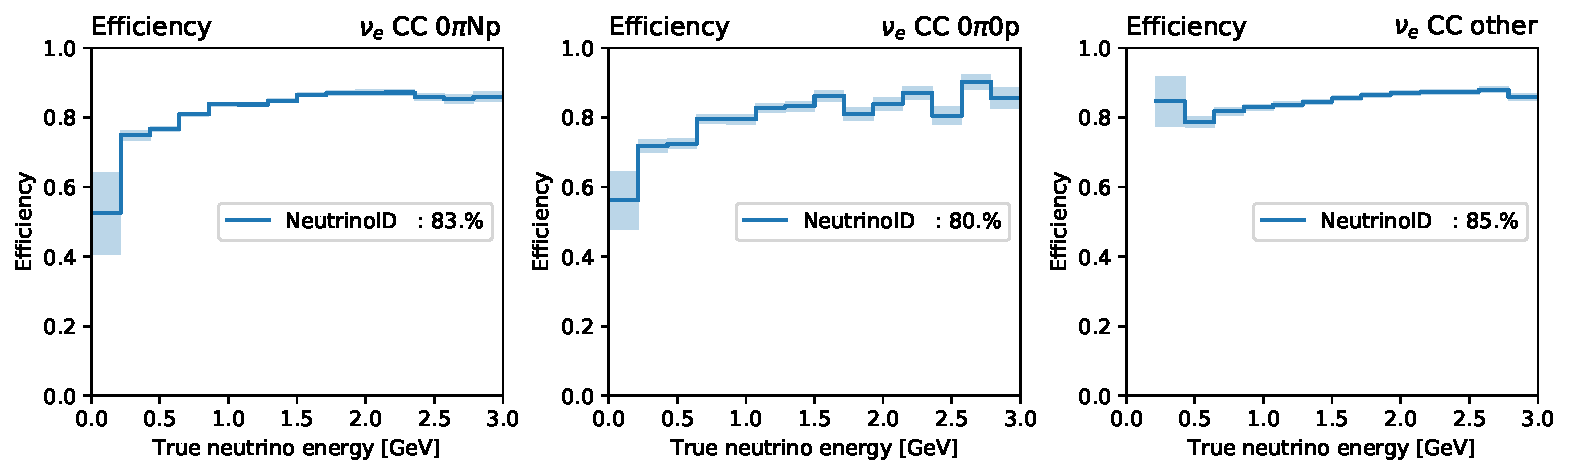
\includegraphics[width=\textwidth]{NuId-Ch2/Images/efficiency_cat_0.pdf}
    \caption{The performance of the SliceID in function of the true neutrino energy for the channel with protons (left), the channel without vertex activity (middle) and events with pions in the final state (right).}
    \label{fig:sliceid}
\end{figure}



\subsection{CRT Veto and Distance Tagger \textcolor{green}{Elena}}
\label{sec:sliceID:CRT}
Contrary to  $\nu_\mu$ interactions and cosmic rays, the charged particles associated to $\nu_e$ interactions are unlikely to deposit energy in the Cosmic Ray Tagger (CRT). Building upon this discriminating factor, the CRT Veto and CRT Distance Tagger are preselection tools which leverage the additional CRT information available for Run 3+ data.
When used, these CRT tools are applied at the pre-selection stage in the following order: CRT Veto, SliceID, CRT Distance Tagger. The CRT tools are especially impactful for the 1e0p channel, where discrimination handles based on the proton PID are obviously missing. \\


\emph{CRT Veto.} %On average, only one in six events passing the MicroBooNE common optical filter is associated to beam-induced activity. The remaining events are triggered by activity that originates outside the TPC: either external beam induced activity or cosmic rays. %Given the $\mathcal{O}(10)$ cosmic ray muons in each drift window, this equates to a starting signal-to-background of $\sim 1 : 60$.
%The CRT Veto looks at CRT activity in time with the beam window. 
The CRT veto looks for a time coincidence between the scintillation light recorded in time with the 1.6 $\mu$s beam-spill (beam-flash) and a CRT hit: if a CRT hit occurs within a 1 $\mu s$ of the beam flash, the event is rejected. For this coincidence, only CRT hits with PE $>$ 100 pe are considered; we do not apply a constraint on the position of the flash nor on the position of the CRT hit. 
The rejection power and efficiency of the CRT veto are calculated using the BNB external and the $\nu_e$ overlay samples, respectively. The BNB external passing rate is $\sim$59\%,  and the $\nu_e$ efficiency greater than $\sim$94\% for all electron neutrino energies, raising at low energies. \\


\emph{CRT Distance Tagger.} 
The CRT Distance Tagger tool builds upon the standard pandora neutrino vertex reconstruction and the CRT tagging of TPC tracks. A TPC track is tagged with a CRT hit association if the track projection onto a CRT panel and a CRT hit are close in space. 
To perform this association, the track projection to the CRT is calculated under the hypothesis that the associated particle crossed the TPC at the time registered by the CRT hit under consideration; more details on the CRT hit to TPC track match are available in \cite{bib:CRTPresel_Technote}.  The CRT Distance Tagger checks the minimum distance between the reconstructed neutrino vertex and each track tagged with a CRT hit. If the minimum distance is less than 14 cm, the event is rejected. An example event tagged by this cut is shown in Figure~\ref{fig:crtdist00}.  For the CRT Distance Tagger, the BNB external passing rate is $\sim$81\%,  and the $\nu_e$ efficiency greater than $\sim$96\% for all electron neutrino energies, raising at low energies. \\
 
\begin{figure}[h!]
\centering
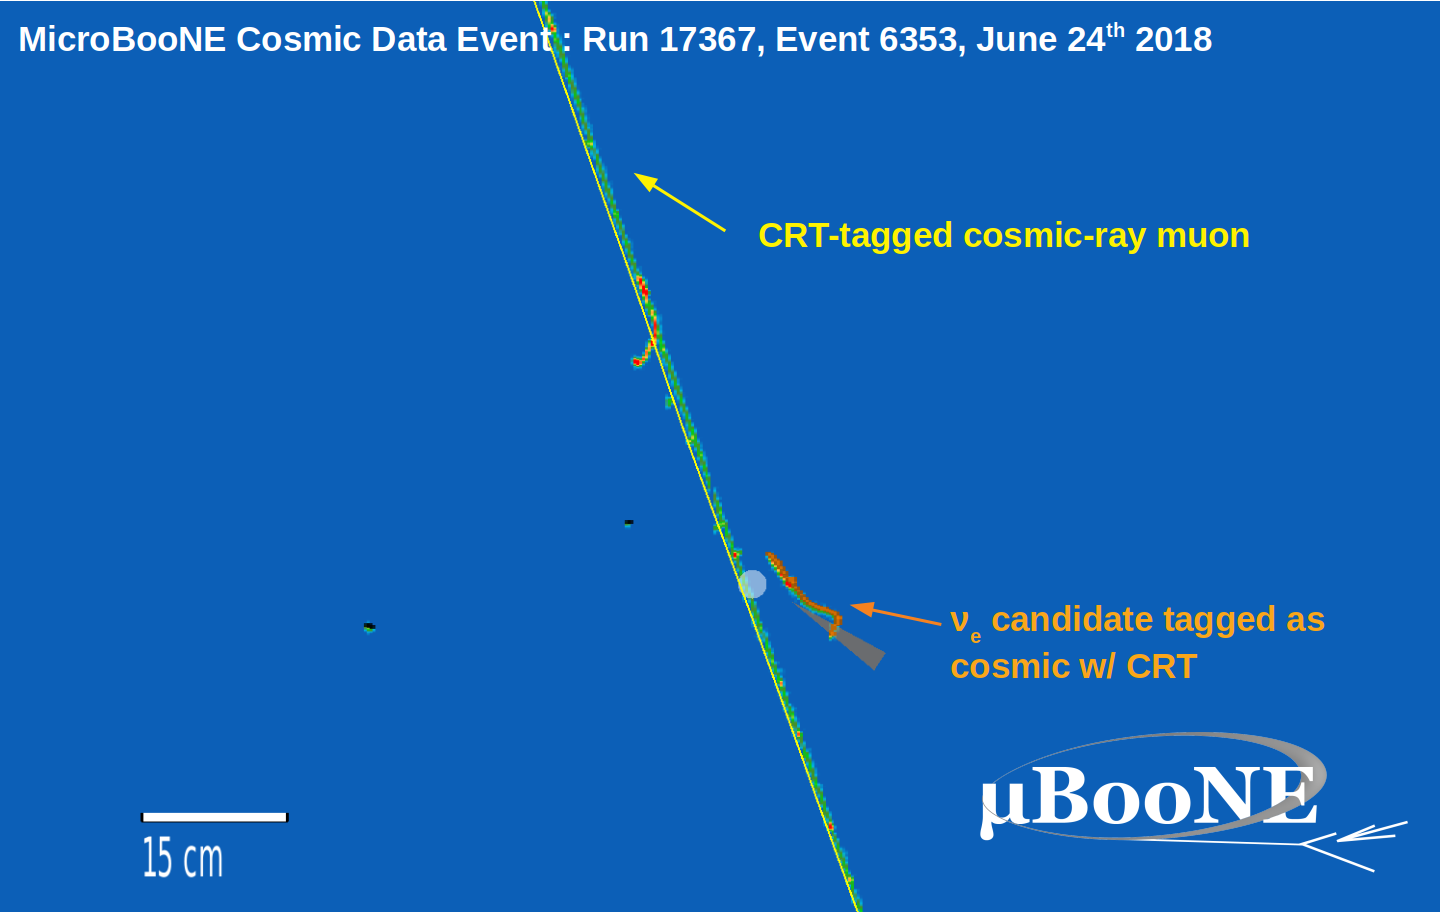
\includegraphics[width=0.4\textwidth]{NuId-Ch2/Images/crttagger_01.png}
\caption{Example $\nu_e$ candidate tagged as cosmic thanks to the CRT distance tagger. From the event one can see that the reconstructed EM shower is associated to EM activity associated to the incoming muon.}
\label{fig:crtdist00}
\end{figure}

An overview of the impact of the CRT on cosmic rejection can be seen in Figure~\ref{fig:crt} where the beam-time distribution for the $8E18$ POT Run 3 open dataset is shown after SliceID (left), and after SliceID and CRT cosmic-tagging tools (both CRT veto and distance tagger) have been applied (right), with EXT backgrounds dropping by more than a factor of 3.
Further details and a preliminary study of the CRT  impact on an electron neutrino preselection can be found in \cite{bib:CRTPresel_Technote}. 

\begin{figure}[ht] 
\begin{center}
    \begin{subfigure}[b]{0.4\textwidth}
    \centering
    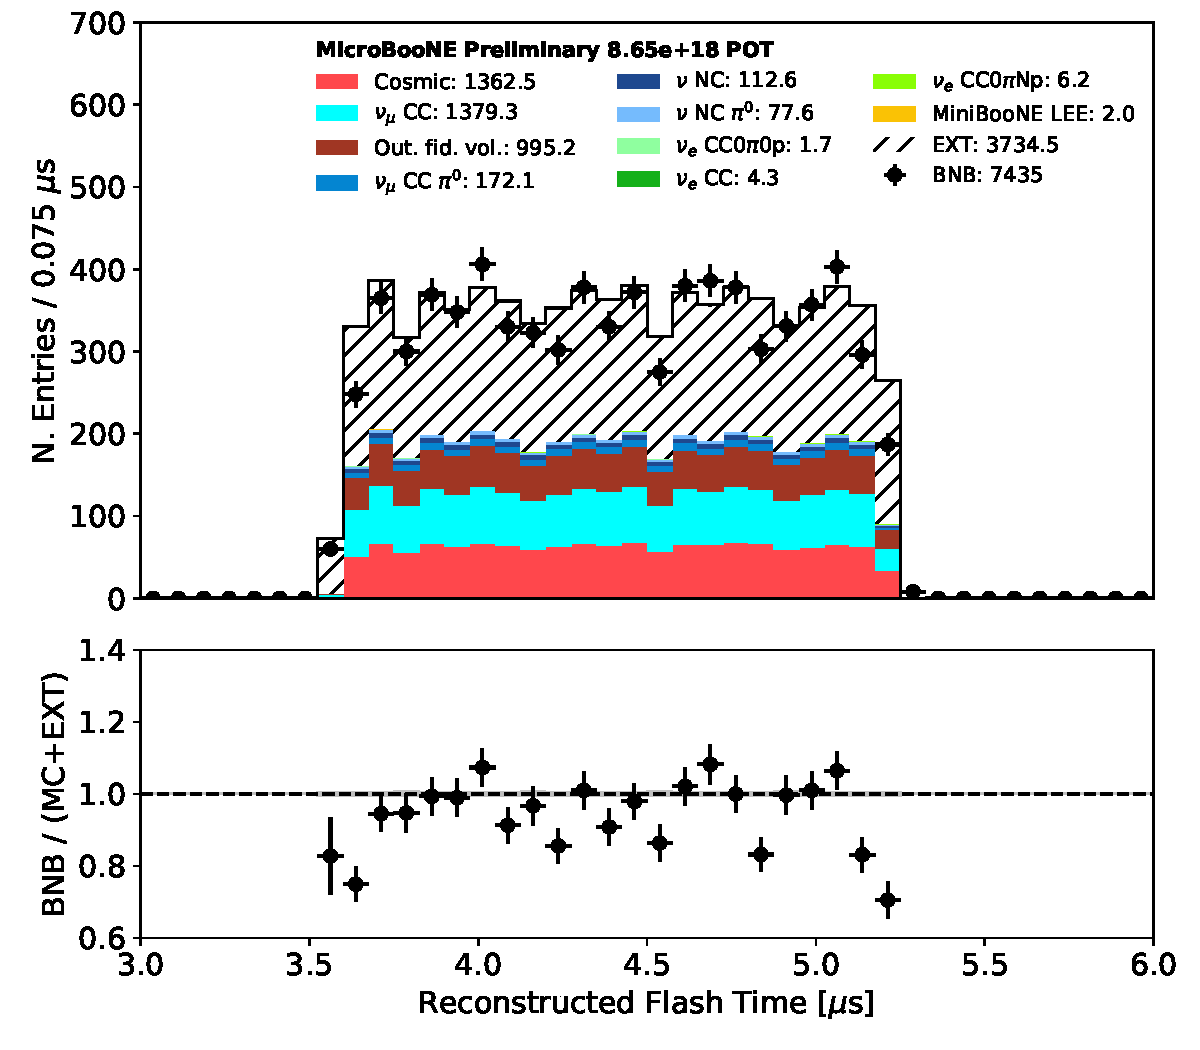
\includegraphics[width=1.00\textwidth]{NuId-Ch2/Images/flash_time_01152020.pdf}
    \caption{\label{fig:crt:pre} no CRT tools.}
    \end{subfigure}
    \begin{subfigure}[b]{0.4\textwidth}
    \centering
    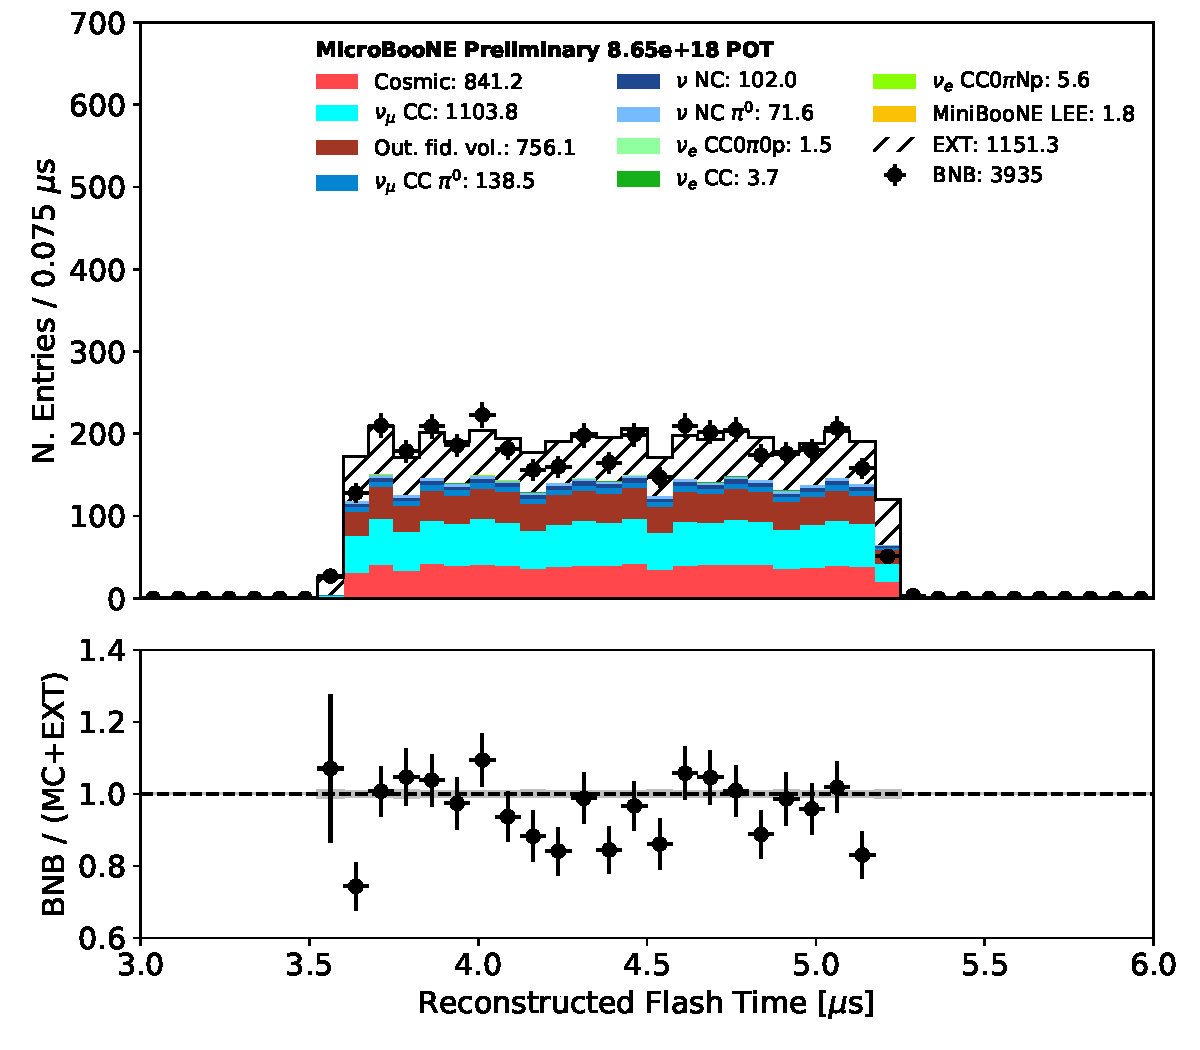
\includegraphics[width=1.00\textwidth]{NuId-Ch2/Images/flash_time_01152020_CRT.pdf}
    \caption{\label{fig:crt:post} with CRT tools.}
    \end{subfigure}
\caption{\label{fig:crt} Beam timing distribution before (left) and after (right) CRT tools have been applied. The EXT contribution is reduced by over a factor of three.}
\end{center}
\end{figure}



\newpage

\section{Neutrino Event Reconstruction \textcolor{red}{Giuseppe, David + ...}}

\subsection{Track and Shower Reconstruction \textcolor{green}{Giuseppe}}
\label{sec:tkshreco}
The output of Pandora~\cite{bib:pandoraub} is organized in a hierarchy of reconstructed Particle Flow Particles (``PFParticles''), which describes the particle content in an observed event as a parent-daughter relationship chain. Final state PFParticles are 3D objects matching clusters of hits in at least two different planes.
Pandora classifies PFParticles as track-like or shower-like base on a Support Vector Machine (SVM) algorithm~\cite{bib:tkshsvm}, producing a score with values between 0 (shower-like) and 1 (track-like).

Pandora processes track-like PFParticles with a sliding linear fit procedure (described in~\cite{bib:pandoraub}) that returns the 3D position and direction at each point along the trajectory (where each point corresponds to a 2D hit). For each point the d$Q$/d$x$ and distance from the track-start are recorded using MicroBooNE's Calorimetry module. This procedure allows to accurately measure d$x$, including small deflections due to the particle's trajectory and SCE offsets, and d$Q$, by incorporating MicroBooNE's full position- and field-dependent relative and absolute charge calibration. From d$Q$/d$x$, d$E$/d$x$ is calculated assuming a fixed recombination correction assuming 2.1 MeV/cm energy loss, but accounting for local variations in the electric field.

We evaluate the energy and 3D direction of shower-like PFParticles with the same algorithm used for the $\pi^0$ reconstruction paper~\cite{bib:pi0reco}. The energy reconstruction accounts for various detector effects, including gain and recombination; corrections for reconstruction effects (hit threshold and imperfect clustering) will be described in Sec.~\ref{sec:ereco}. We also fit showers using a Kalman filter-based procedure~\cite{bib:shrtrackfitter} which aims at identifying the main trunk of the shower by rejecting hits that are longitudinally or transversely displaced from it; the output of this fit is a track object so that the calorimetric tools described above become available for showers as well.

By default, Pandora separates showers and tracks with a cut on the SVM score at 0.5; however, as will be described in later sections, in many cases we choose different cut values, i.e. tighter shower definition for the $\nu_e$ selection and looser for the pi0 control region.

\subsection{Particle Identification \textcolor{green}{Nico}}
% GC: this part is now in the previous subsection
%In the neutrino slice, every PFParticle is reconstructed in three different ways:
%\begin{itemize}
%    \item Track, using the standard Pandora Track reconstruction
%    \item Shower, using the standard Pandora Shower reconstruction (is there any modification on top of this?)
%    \item Track-fitted shower, using a dedicated track fitting tool which aims at identifying the main branch of %the shower and fit it as a track. As a result, all the tools developed for the track become available for the %tracks too. For example, for each track-fitted shower, a recob::track and a anab::calorimetry objects are available.
%\end{itemize}
Particle identification is performed with different tools depending the type of candidate a given PFParticle has been selected as.
If the PFParticle has been selected as a muon or proton candidate, so as a track-like object, the identification is performed using the Calorimetry Likelihood tool, which results in the variable Log Likelihood Ratio PID \ref{subsec:loglikelihoodpid}.
If the PFParticle has been selected as an electron or photon candidate, the identification is performed using several variables described in \ref{subsec:egammaspearation}.

It is noteworthy that this particle identification consists of one or multiple variables, available for the specific PFParticle, that may or may not depend on the rest of the slice. 
For example, the shower dE/dx depends only on the PFParticle itself, whereas the track-shower separation relies also on additional objects identified in the slice.

The value of the cuts applied on these variables depend not only on the general level of efficiency and mis-identification one may want to achieve in distinguishing two kind of particles (electrons from photons, for example), but also on the mixture of backgrounds, which eventually depends on the specific selection the analyser is performing.

\subsubsection{Log Likelihood Ratio Particle ID \textcolor{red}{Nico}}
\label{subsec:loglikelihoodpid}


\subsubsection{$e$/$\gamma$ Separation}
\label{subsec:egammaspearation}
\par Distinguishing electron from photon EM-showers is one of the crucial steps required to perform a measurement of $\nu_e$ interactions in the BNB beam. Photon backgrounds to a $\nu_e$ measurement are largely caused by neutrino interactions with $\pi^0 \rightarrow \gamma\gamma$ in the final state, which dominate the $\nu_e$ event rate by at least an order of magnitude. Three key features distinguish events with $\pi^0$ induced photon showers from $\nu_e$ interactions: (a) the presence of two final state EM showers. (b) the non-zero conversion distance separating the neutrino interaction vertex from the shower start point, and (c) the calorimetric separation via $dE$/$dx$ due to the overlapping ionization segment of $e^+$/$e^-$ pair-conversions through which most $\gamma$ showers manifest themselves. Figure~\ref{fig:egammasep} shows how, at reconstruction level, each of these features can aid in $e$/$\gamma$ separation. This section describes how each of the items above is utilized in the analysis on a technical level, what performance is obtained and challenges (both physics- and reconstruction-driven) are encountered in doing so.

\begin{figure}[ht] 
\begin{center}
    \begin{subfigure}[b]{0.31\textwidth}
    \centering
    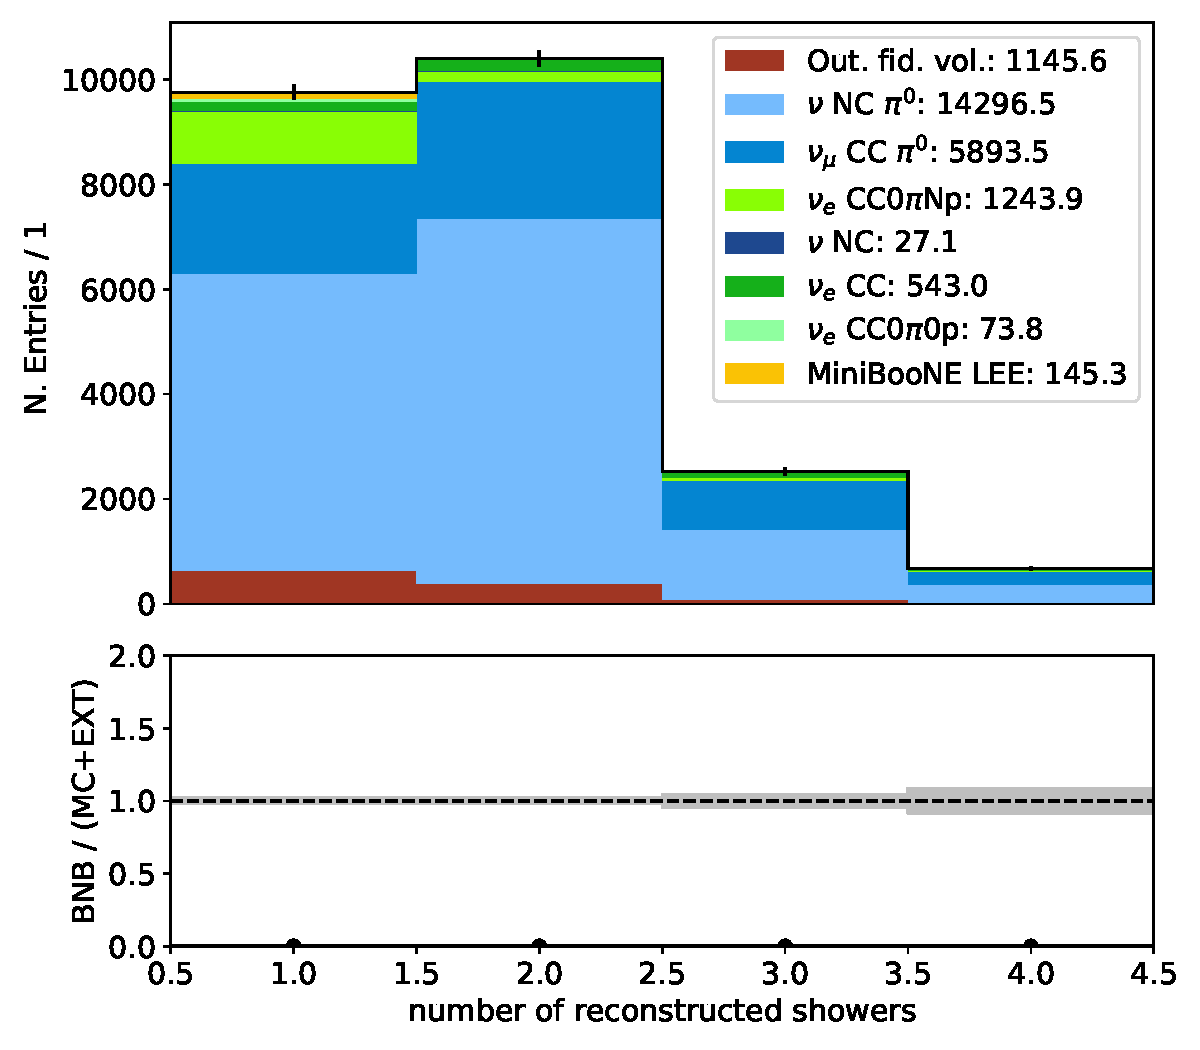
\includegraphics[width=1.00\textwidth]{egamma/n_showers_contained_01022020.pdf}
    \caption{number of reconstructed showers}
    \end{subfigure}
    \begin{subfigure}[b]{0.31\textwidth}
    \centering
    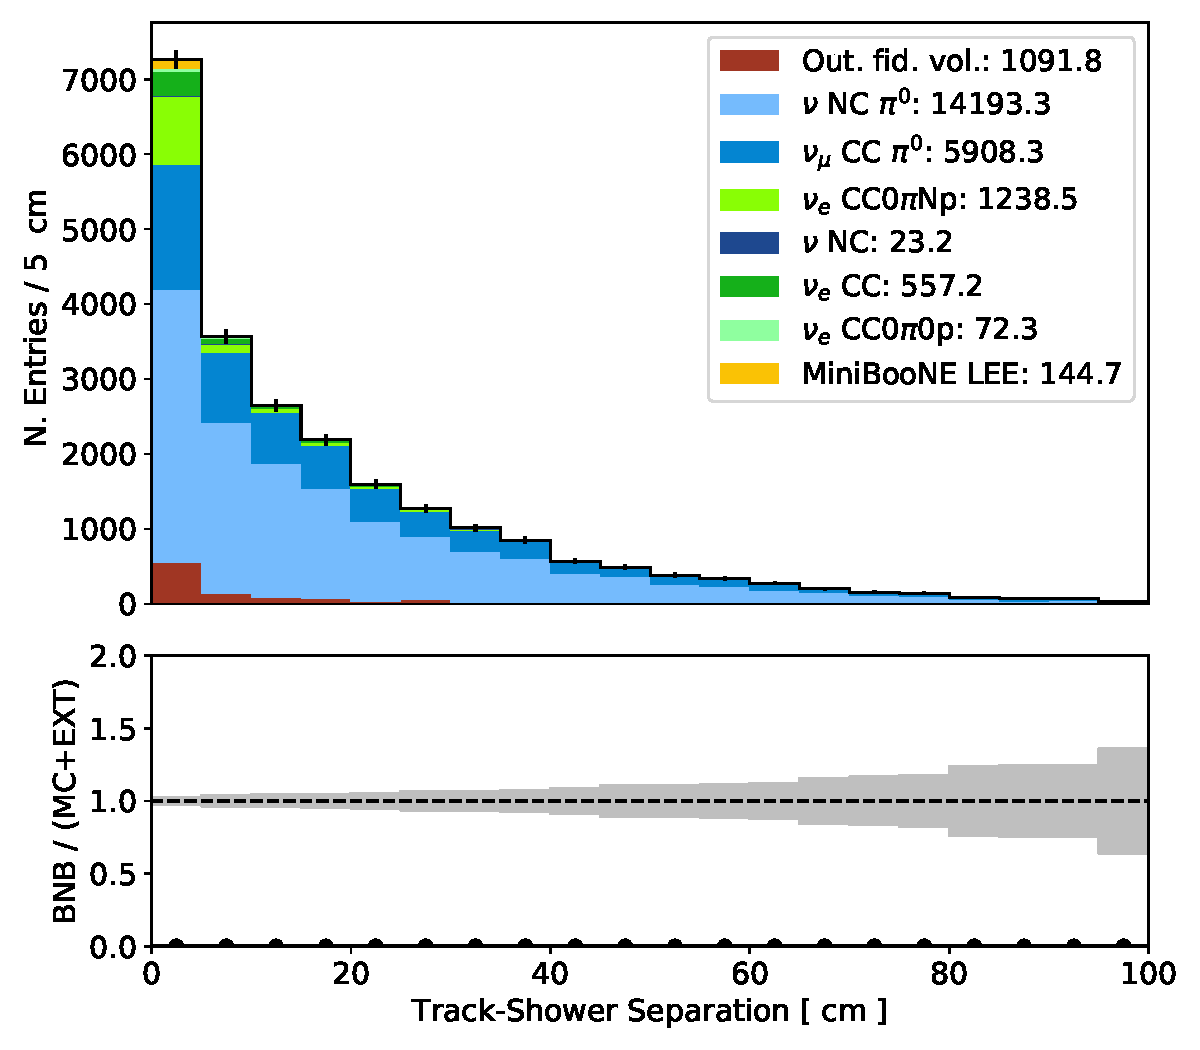
\includegraphics[width=1.00\textwidth]{egamma/tksh_distance_01022020.pdf}
    \caption{track-shower separation}
    \end{subfigure}
    \begin{subfigure}[b]{0.31\textwidth}
    \centering
    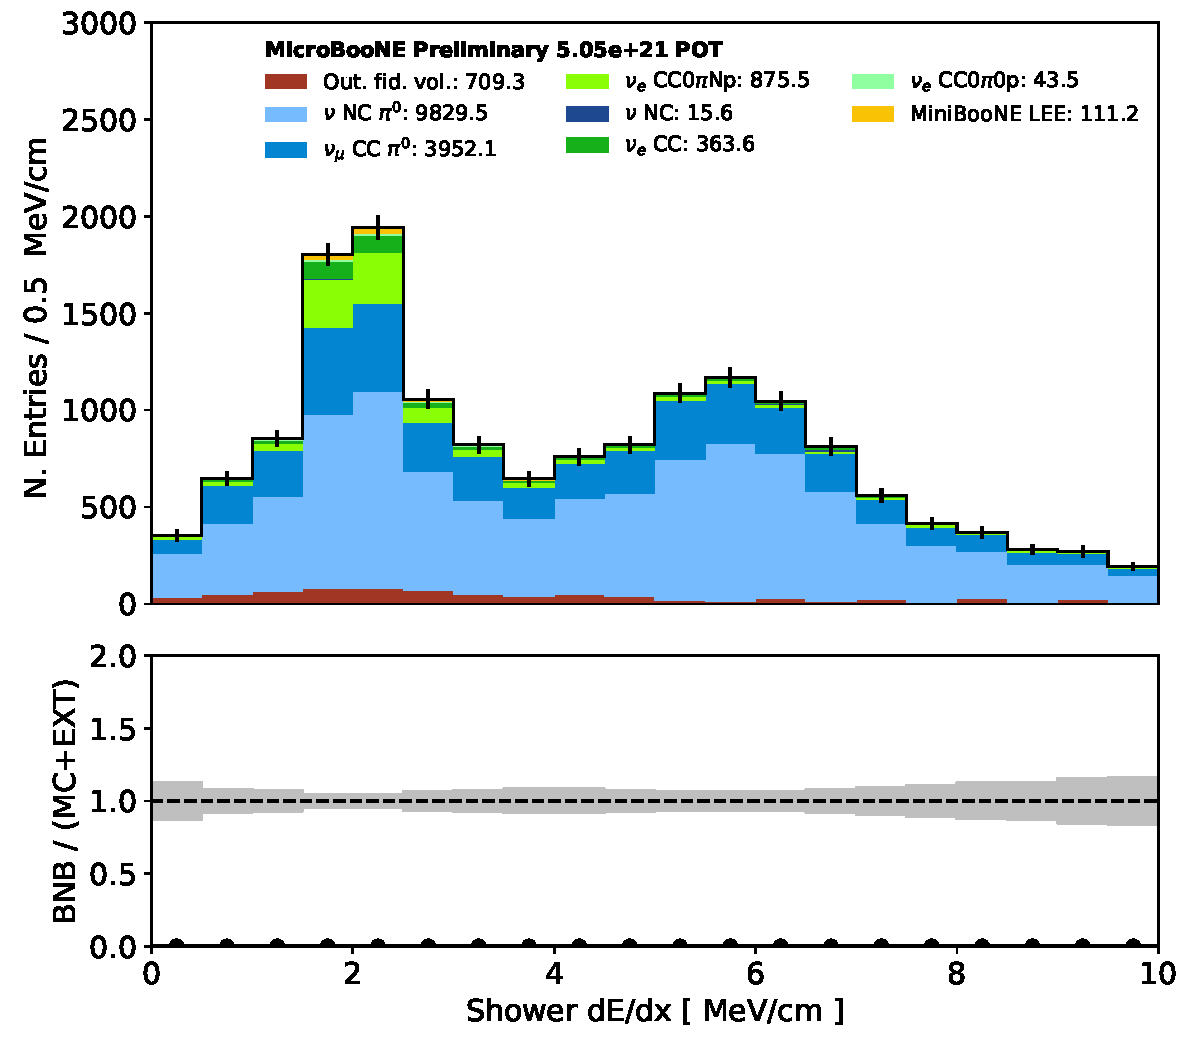
\includegraphics[width=1.00\textwidth]{egamma/shr_tkfit_dedx_Y_01022020.pdf}
    \caption{\label{fig:egammasep:dedx} reconstructed shower $dE$/$dx$}
    \end{subfigure}
\caption{\label{fig:egammasep}Comparison of simulated $\nu_e$ (green) vs. $\nu_{\mu} \rightarrow \pi^0 + X$ (blue) for the three discriminating variables of (a) number of showers, (b) vertex distance, and (c) $dE$/$dx$. Distributions are POT-normalized but do not conatain non-$\nu_e$ or non-$\pi^0$ events, nor on/off-beam data distributions.}
\end{center}
\end{figure}

\par \textbf{two-shower requirement} Requiring a single reconstructed shower keeps 68\% of $nu_e$ interactions (with no $\pi^0$ in the final state) while removing 61\% of $\nu_{\mu}$ events with at least one $\pi^0$ in the final state. The fraction of kept $\nu_e$s grows to 79\% when looking below 800 MeV of true energy (the focus of this analysis). Rejection of $\nu_e$s is largely due to events where the electron shower is reconstructed as two separate EM showers, often closely aligned in 3D. Events with final state $\pi^0$s are reconstructed with a single EM shower in the final state because either the second photon escapes the TPC active volume completely (irreducible) or because the second shower is not reconstructed. The dominant causes of this second case are (1) highly-boosted $\pi^0$ decays, in which two aligned photons are merged into one shower and (2) photons which go undetected, often low in energy (below 100 MeV). Additional discriminating variables which aim to recover the reconstruction-related mis-ID of (1) and (2) are utilized in the analysis and presented in Sec.~\ref{sec:nueselection:tools}.
\par \textbf{track-shower separation} For events where hadronic activity at the neutrino interaction vertex (i.e. final-state protons) is visible, a clear gap between the vertex and the shower start-point can be used to reject $\gamma$ backgrounds. This is a powerful background mitigation tool in the 1$e$N$p$ $\nu_e$ selection. Two factors determine the performance of such a tool: the ability to detect protons and other hadronic activity at the vertex and the accuracy with which the shower start-point is reconstructed. The shower start-point reconstruction accuracy determines the level of background rejection one can obtain, as $\gamma$ showers lead to an exponential conversion-distance distribution. A 1 vs. 5 cm track-shower separation cuts lead to 95\% vs 74\% mis-ID respectively, but causes a drop in selection efficiency for 1$e$N$p$ events from 72\% to 28\%. In order to enhance the ability to isolate $\nu_e$ events in the 1$e$N$p$ selection through vertex-displacement, different metrics are used to measure the presence of a gap between an electron and proton candidate. These will be described in section~\ref{sec:nueselection:tools}. It is important to note that this background mitigation strategy is not applicable to single-electron searches, which are an important contribution to $\nu_e$ interactions, especially in the low-energy regime.
\par \textbf{shower d$E$/d$x$} The majority of photons manifest themselves in a TPC through the ionization released by the $e^+$/$e^-$ pair produced via pair-conversion. The electron-positron pair is highly aligned and overlaps on the mm-scale, leading to a doubly-ionizing charge-segment compared to electron showers. To measure this, we use the track fit of the main shower trunk and the calorimetric tools as described in Sec.~\ref{sec:tkshreco}. 
%with a modified version of the MicroBooNE track-fitter~\cite{bib:shrtrackfitter} and for each point along a track the d$Q$/d$x$  and distance from the shower-start are recorded using MicroBooNE's Calorimetry module. This procedure allows to accurately measure d$x$, including small deflections due to the electron's trajectory and SCE offsets, and d$Q$, by incorporating MicroBooNE's full position- and field-dependent relative and absolute charge calibration. From d$Q$/d$x$, d$E$/d$x$ is calculated assuming a fixed recombination correction assuming 2.1 MeV/cm energy loss, but accounting for local variations in the electric field. 
The distinctive 4 MeV/cm population expected for $\gamma$ showers is visible in figure~\ref{fig:egammasep:dedx}. The main limitation to $e$/$\gamma$ separation via d$E$/d$x$ is the large fraction of photons reconstructed with a d$E$/d$x$ of less then 3 MeV/cm (23\% of $\pi^0$ events fall in the 1-3 MeV range). This is due both to mis-reconstructed events, for which the start-point is incorrectly reconstructed by more than one or two cm, and to events where the photon shower's energy loss-profile is not as clearly distinguishable from that of a single electron. While the relative contribution of these two sources is still under determination, the second causes a significant mis-ID rate, and is largely associated to lower-energy $\gamma$ showers for which the production of a highly asymmetric electron-positron pair where one of the electrons is barely visible is more frequent. The impact of shower energy on the measured d$E$/d$x$ for a $\gamma$ shower is shown in figure~\ref{fig:dedxgammas:energy}. Below 100 MeV, where most $\gamma$ showers in the BNB are produced, the reconstructed d$E$/d$x$ is electron-like. The impact of distance from the shower start-point on whether d$E$/d$x$ is reconstructed to be 2 or 4 MeV/cm is also important, as can be seen in figure~\ref{fig:dedxgammas:dist}. This is particularly true for low-energy asymmetric pair-production events, and motivates utilizing 
d$E$/d$x$ information at different distances from the shower start-point for $e$/$\gamma$ separation.
\begin{figure}[H] 
\begin{center}
    \begin{subfigure}[b]{0.45\textwidth}
    \centering
    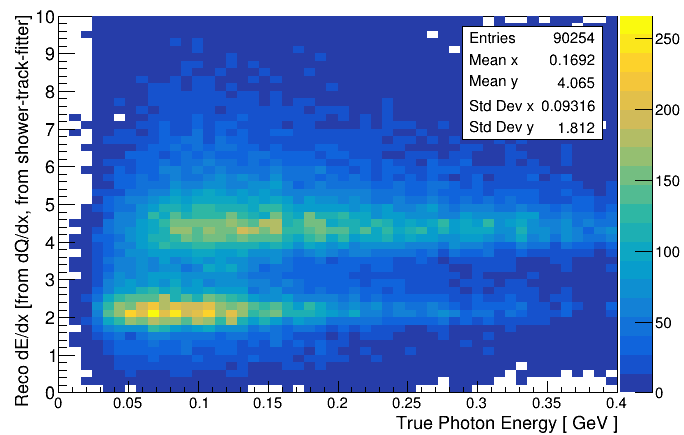
\includegraphics[width=1.00\textwidth]{egamma/dedx_vs_energy_gamma.png}
    \caption{\label{fig:dedxgammas:energy} d$E$/d$x$ vs. distance from shower start-point for $\gamma$ showers}
    \end{subfigure}
    \begin{subfigure}[b]{0.45\textwidth}
    \centering
    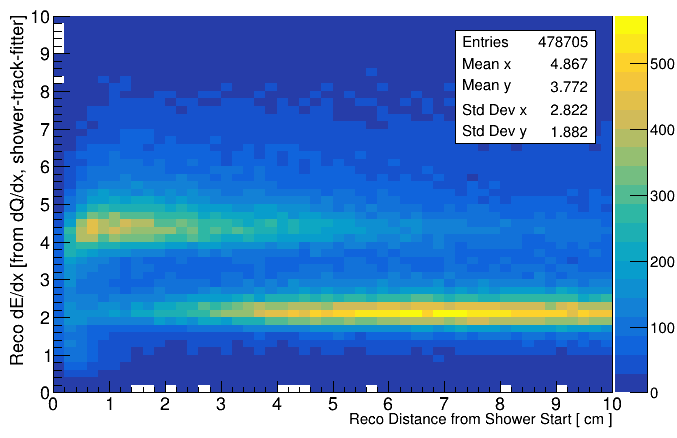
\includegraphics[width=1.00\textwidth]{egamma/dedx_vs_dist_gamma.png}
    \caption{\label{fig:dedxgammas:dist} d$E$/d$x$ vs. distance from shower start-point for $\gamma$ showers}
    \end{subfigure}
\caption{\label{fig:dedxgammas}}
\end{center}
\end{figure}

\newpage

\subsection{Energy Reconstruction \textcolor{red}{Giuseppe + David}}
\label{sec:ereco}
\par Energy reconstruction is performed calorimetrically for EM showers and through a measurement of a track's range for contained muons and protons. For muons multiple Coulomb scattering (MCS) is also used to estimate the muon energy. The energy resolution obtained for different particles is reported in table~\ref{tab:eres}. More information on each particle specie's energy resolution is reported in figure~\ref{fig:eres:particle} where for each particle species the 2D reconstructed vs. true energy distribution (in log-scale) is shown on the left, next to a plot of energy resolution vs. true energy on the right. The energy resolution reported here is obtained from a Gaussian plus one-sided exponential fit to the distribution $[E_{\rm reco}-E_{\rm true}] / E_{\rm true}$. The resolution reported refers only to the Gaussian width $\sigma$ extracted in the fit, and therefore does not account for negative tails, which are significant in the case of EM shower energy reconstruction, and described below.


\begin{table}[H]
\centering
  \begin{tabular}{ | c | c |  }
    \hline
    particle & kinetic energy resolution  \\ \hline
    proton & 4\% at 100 MeV 1\% at 200 MeV \\ \hline
    muon (range) & 3\%  \\ \hline
    muon (MCS) & $\frac{4.7\%}{\sqrt{E/{\rm GeV}}} \otimes \frac{2.8\%}{E/{\rm GeV}} \otimes 0.0\%$  \\ \hline
    electron & 15\%  \\
    \hline
    
  \end{tabular}
  \caption{\label{tab:eres} Energy resolution for different particle species.}
 \end{table}
 
 \par For EM showers, the calorimetric energy reconstruction response has a significant non-Gaussian component, as well as a large bias. Both effects are attributable to reconstruction effects associated with under-clustering of charge. The energy bias is found to be 20\% and approximately flat in energy, and motivates a definition of a corrected shower energy, defined as $E_{\rm corrected} = E_{\rm calorimetry} / 0.8$. The non-Gaussian response for EM energy reconstruction can be modeled through a Gaussian plus one-sided exponential distribution. Figure~\ref{fig:eres:elec:binned} shows in different bins of true energy the fractional energy response and a fit to a Gaussian plus one-sided exponential function. The residual energy bias, after the 20\% correction applied, is of order $3-8$\%. 
 
 \begin{figure}[ht]
\begin{center}
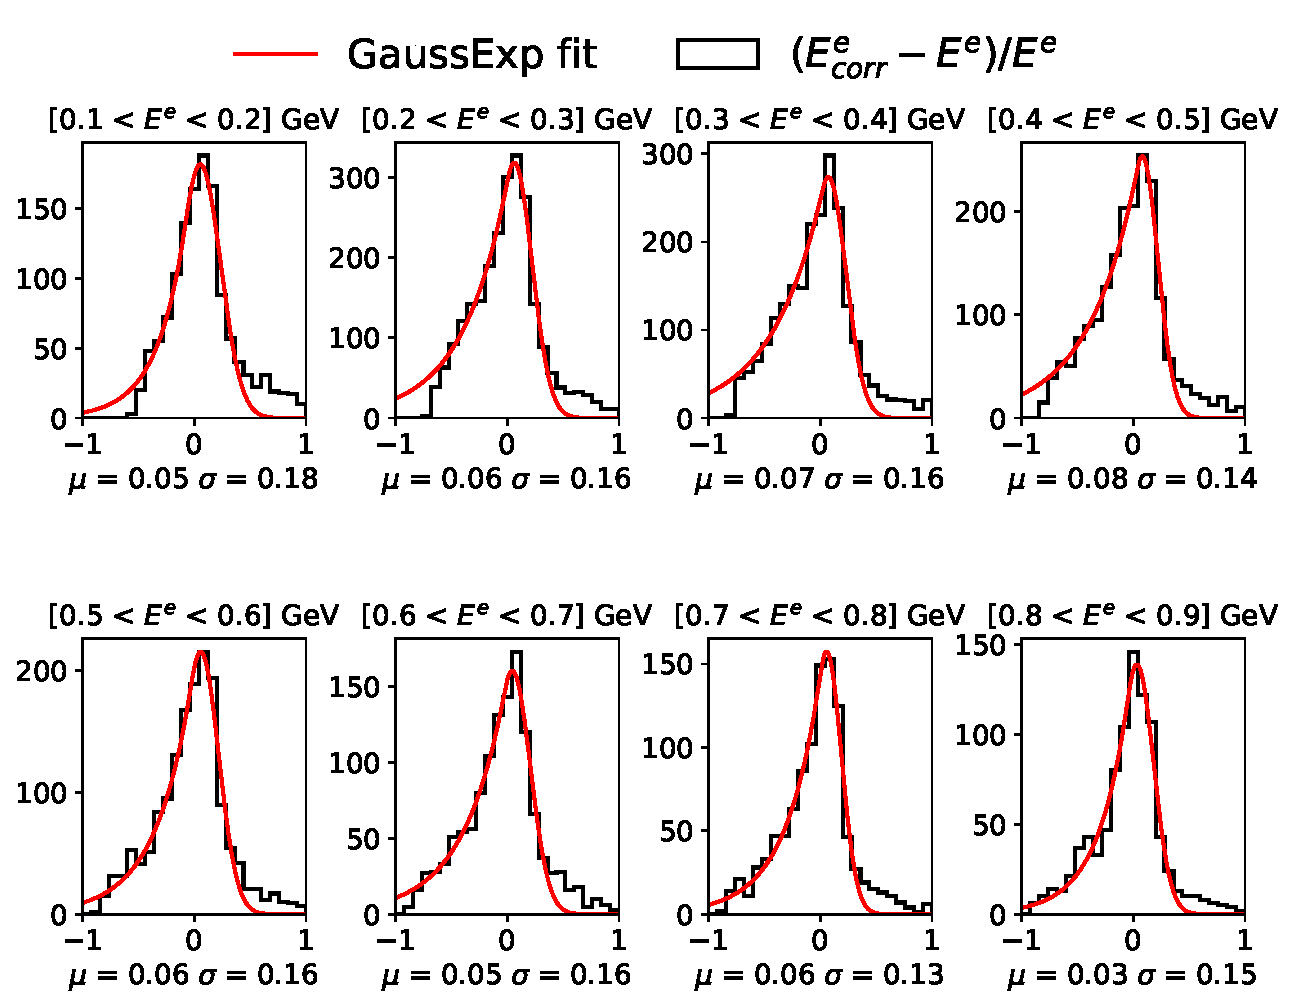
\includegraphics[width=0.75\textwidth]{ereco/elec_eres_binned.pdf}
\caption{\label{fig:eres:elec:binned}Energy resolution for electron showers.}
\end{center}
\end{figure}
 
 \newpage

\begin{figure}[H] 
\begin{center}
    \begin{subfigure}[b]{0.4\textwidth}
    \centering
    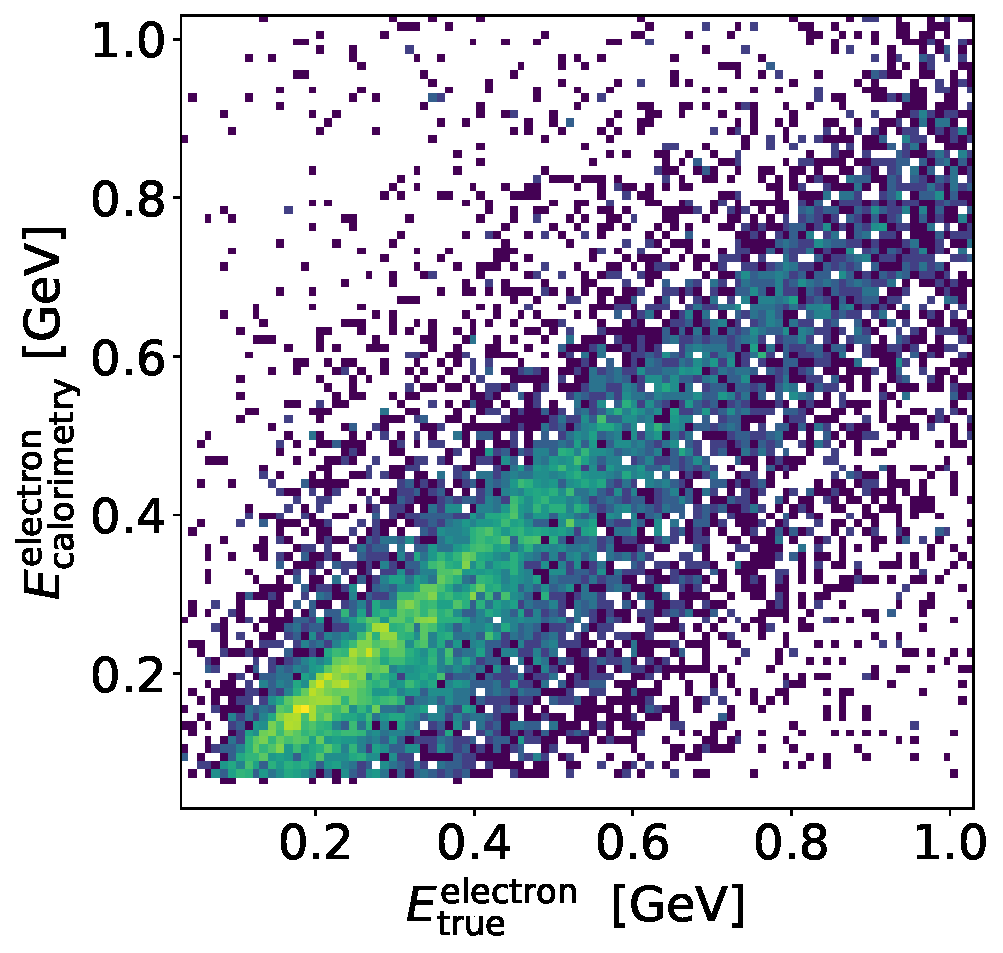
\includegraphics[width=1.00\textwidth]{ereco/electron_eres2D.pdf}
    %\caption{\label{fig:eres:elec:2d} }
    \end{subfigure}
    \begin{subfigure}[b]{0.38\textwidth}
    \centering
    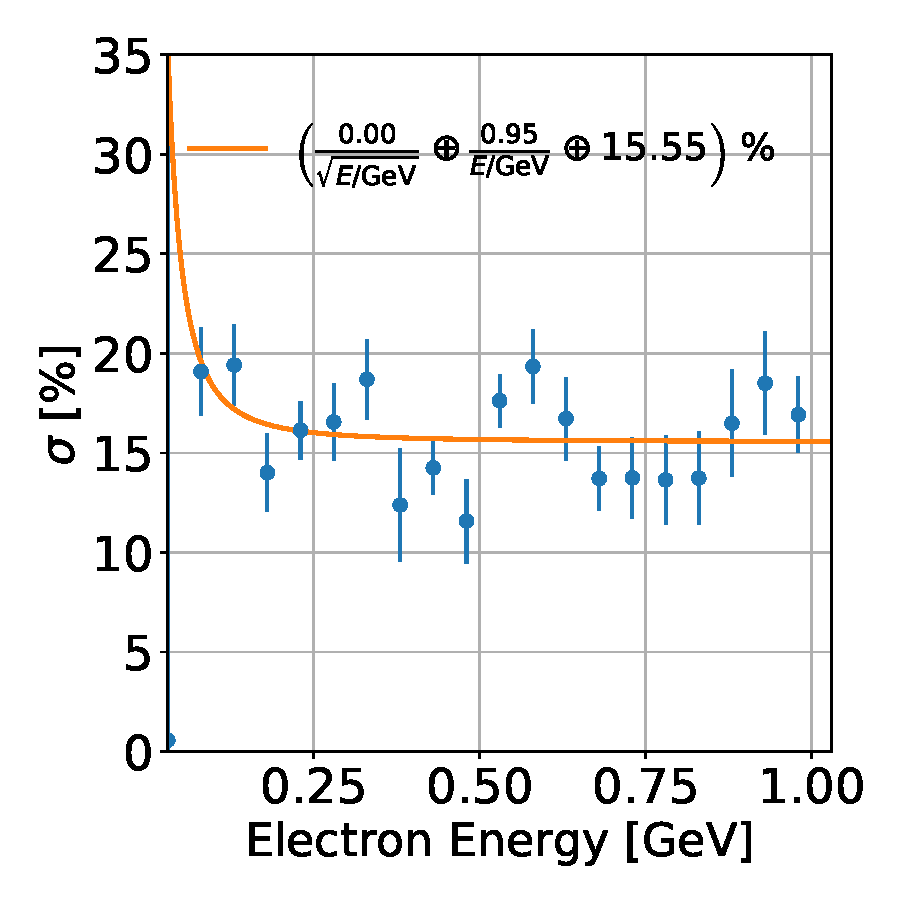
\includegraphics[width=1.00\textwidth]{ereco/elec_eres_vs_true.pdf}
    %\caption{\label{fig:eres:elec:vstrue} }
    \end{subfigure}
    \begin{subfigure}[b]{0.4\textwidth}
    \centering
    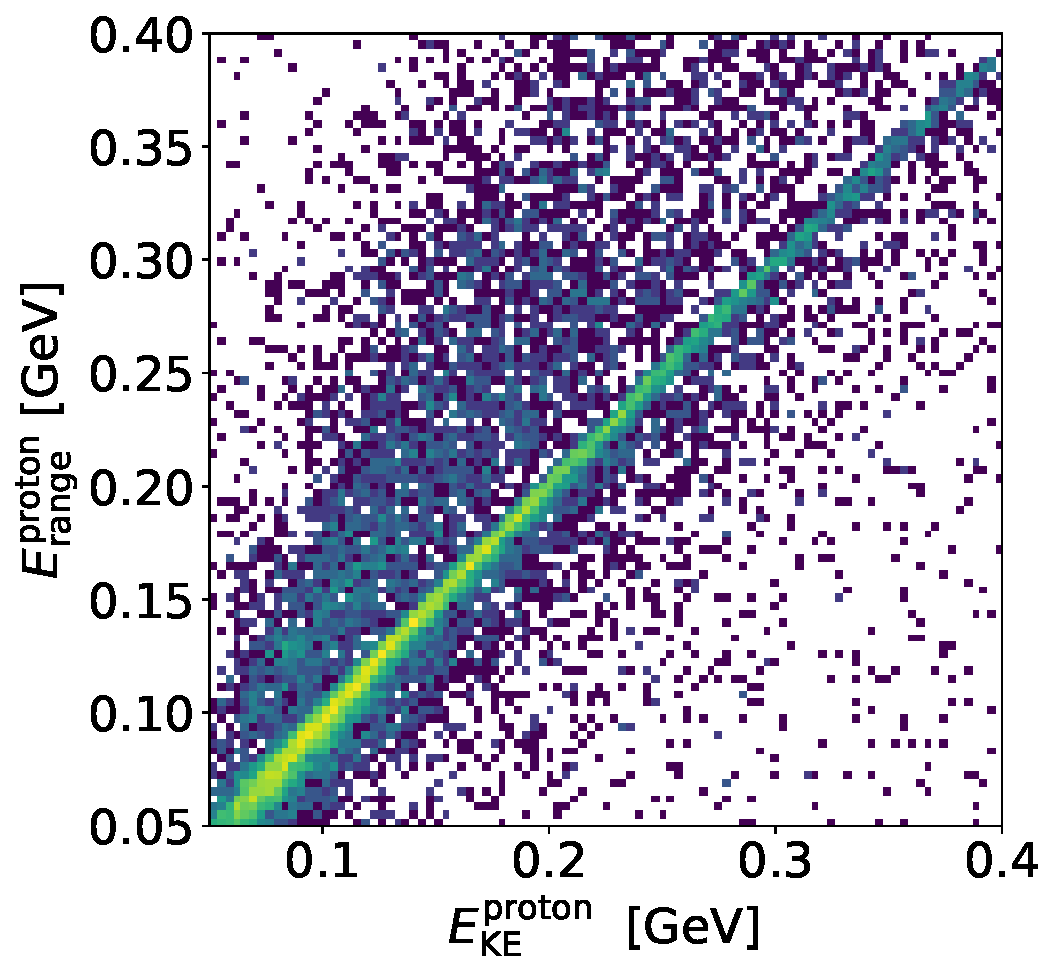
\includegraphics[width=1.00\textwidth]{ereco/proton_eres2D.pdf}
    %\caption{\label{fig:eres:proton:2d} }
    \end{subfigure}
    \begin{subfigure}[b]{0.38\textwidth}
    \centering
    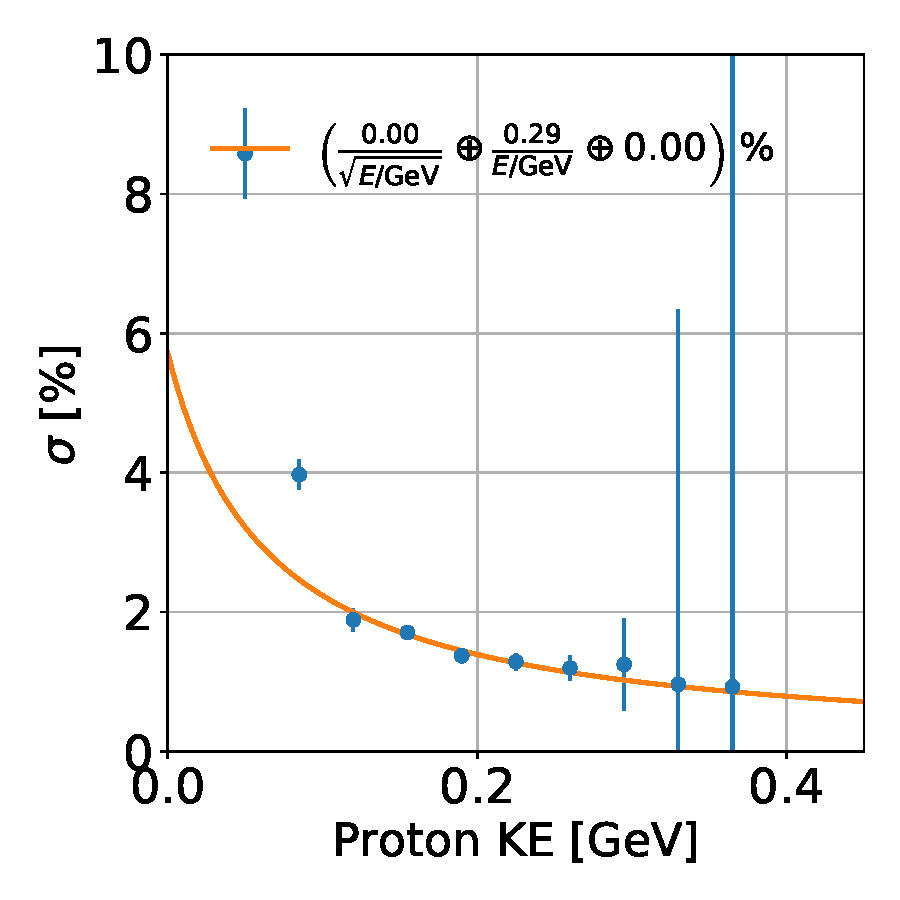
\includegraphics[width=1.00\textwidth]{ereco/proton_eres_vs_true.pdf}
    %\caption{\label{fig:eres:proton:vstrue} }
    \end{subfigure}
    \begin{subfigure}[b]{0.4\textwidth}
    \centering
    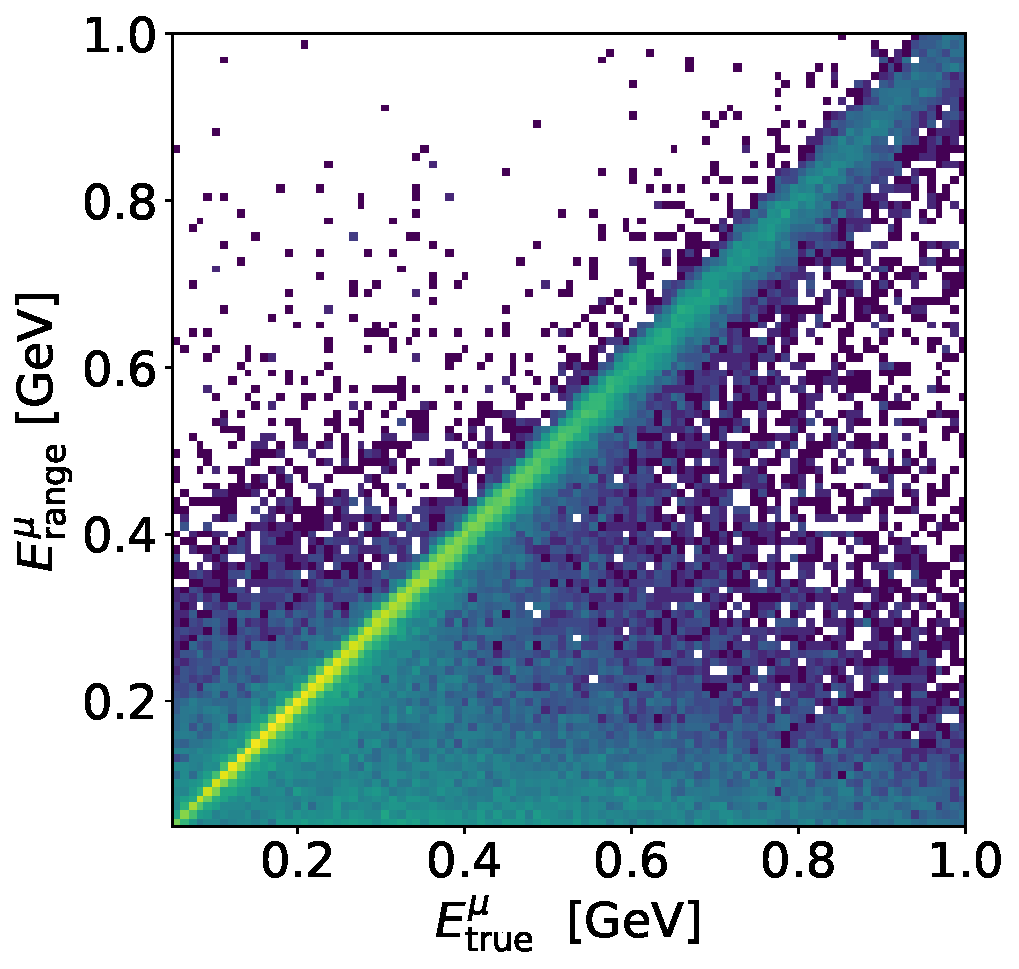
\includegraphics[width=1.00\textwidth]{ereco/muon_range_eres2D.pdf}
    %\caption{\label{fig:eres:muon:2d} }
    \end{subfigure}
    \begin{subfigure}[b]{0.38\textwidth}
    \centering
    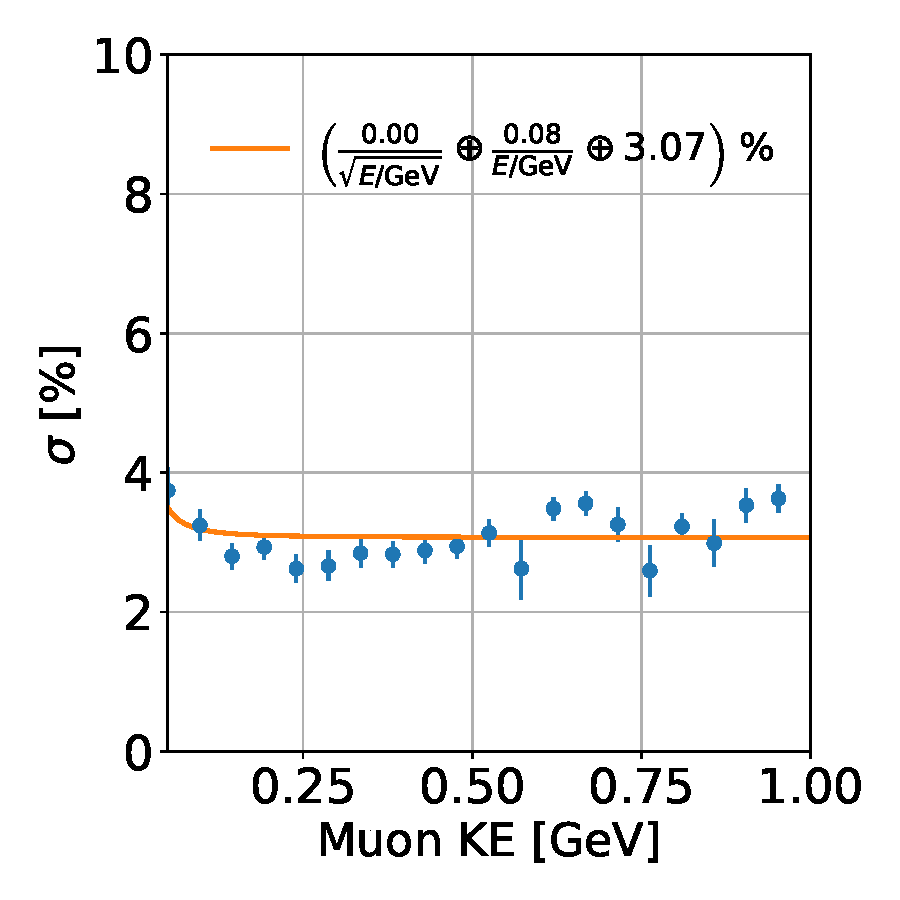
\includegraphics[width=1.00\textwidth]{ereco/muon_range_eres_vs_true.pdf}
    %\caption{\label{fig:eres:muon:vstrue} }
    \end{subfigure}
\caption{\label{fig:eres:particle}Energy resolution for electrons (top), protons (center) and muons (bottom). Left: reconstructed vs. true energy resolution (log-scale). Right: energy resolution from Gaussian fit to $[E_{\rm reco}-E_{\rm true}] / E_{\rm true}$.}
\end{center}
\end{figure}

\newpage

\subsubsection{Neutrino Energy Reconstruction}

\par In this analysis, the energy reconstruction for neutrino interactions is performed through a sum of the visible energy of the various reconstructed final-state particles in the interaction. For $\nu_e$ events the reconstructed energy is defined as:
\begin{equation}
    E_{\rm reco}^{\nu_e} = E_{\rm corrected}^{\rm electron} + \sum_{\rm tracks} E_{\rm range}^{\rm proton}
\end{equation}{}

For contained $\nu_{\mu}$ interactions, the reconstructed energy is defined as:

\begin{equation}
    E_{\rm reco}^{\nu_{\mu}} = E_{\rm range}^{\rm muon} + \sum_{\rm protons} E_{\rm range}^{\rm proton} + 0.105 \; GeV
\end{equation}{}

Figure~\ref{fig:eres:neutrino} shows the comparison between reconstructed energy and truth visible energy, which is defined as the sum of the lepton energy, pion energy (if present), and proton energy (for all protons above 40 MeV of KE). This comparison shows very accurate energy reconstruction for $\nu_{\mu}$ events. For $\nu_e$ interactions, with smearing dominated by the worse energy resolution of electron showers.

\begin{figure}[H] 
\begin{center}
    \begin{subfigure}[b]{0.4\textwidth}
    \centering
    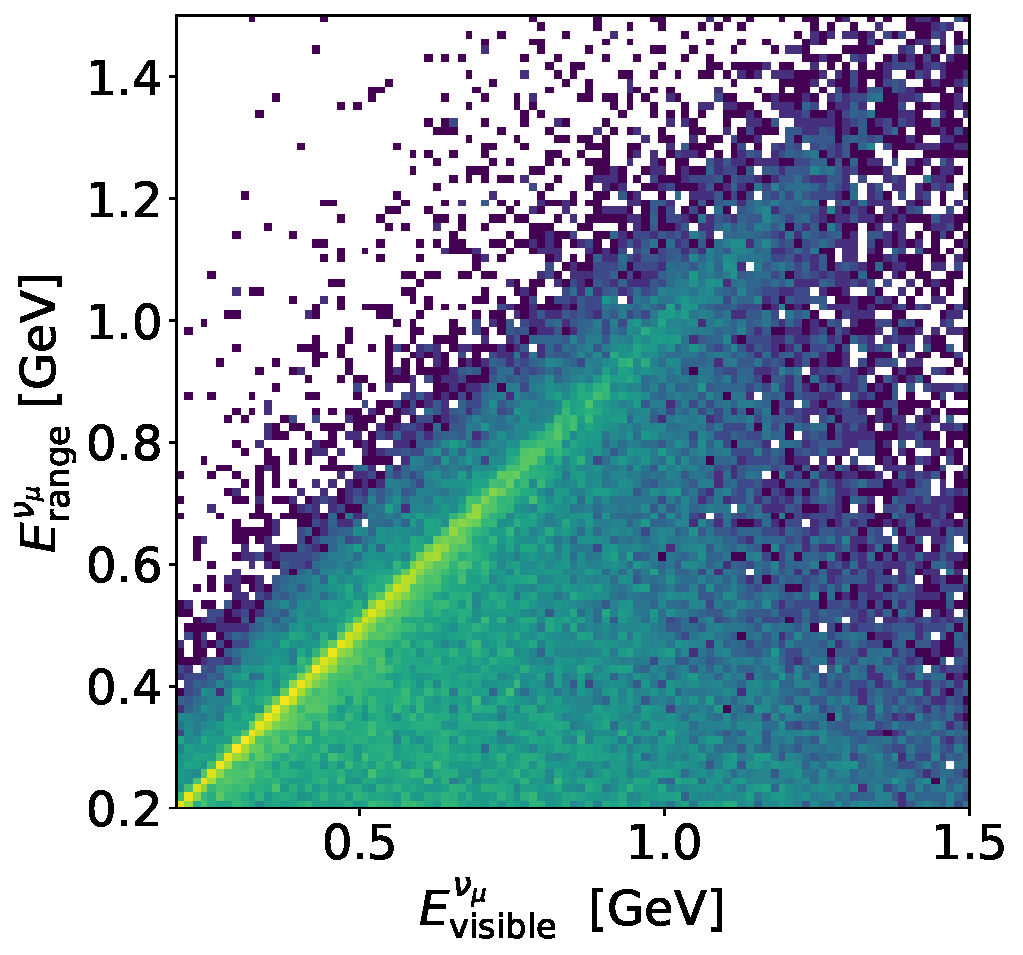
\includegraphics[width=1.00\textwidth]{ereco/numu_energy_visible_eres2D.pdf}
    \caption{\label{fig:eres:numu:2d} }
    \end{subfigure}
    \begin{subfigure}[b]{0.4\textwidth}
    \centering
    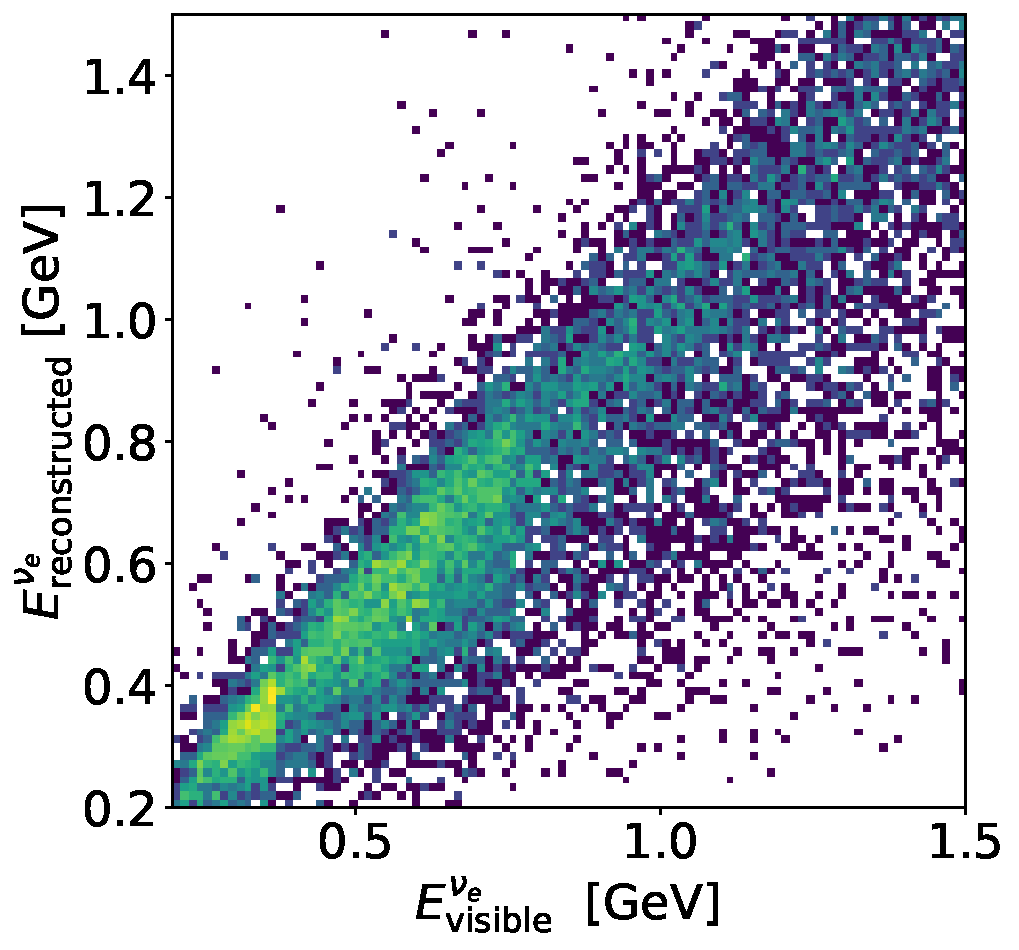
\includegraphics[width=1.00\textwidth]{ereco/nue_visible_eres2D.pdf}
    \caption{\label{fig:eres:nue:vstrue} }
    \end{subfigure}
\caption{\label{fig:eres:neutrino}Log-scale color-maps.}
\end{center}
\end{figure}

\newpage

\section{$\nu_e$ Selections}

\subsection{Common Tools and Inputs \textcolor{red}{Sophie + ...}}
\label{sec:nueselection:tools}

The 1$e$N$p$ and 1$e$0$p$ selections rely on a common pre-selection which requires the presence of at least one reconstructed and contained EM shower (figure~\ref{fig:nue:presel:nshower}) with reconstructed energy above 70 MeV (figure~\ref{fig:nue:presel:shrenergy}). This second cut applies as a Michel-electron veto, as the majority of events which do not pass this cut are associated to cosmic or $\nu_{\mu}$ induced $\mu \rightarrow e$ Michel electrons. The two selections are subsequently split based on whether a proton candidate is (N$p$) or is not (0$p$) found. Events with a fully contained track must have a \texttt{trkpid} score $< 0$ and a value of \texttt{tksh\_angle} $> -0.9$. The first condition requires that the track be proton-like according to the PID tool~\ref{subsec:loglikelihoodpid}, while the second excludes tracks reconstructed back-to-back to the electron candidate, generally due to mis-reconstruction. For events with more than one reconstructed track, these requirements are applied on the longest track.

\begin{figure}[H] 
\begin{center}
    \begin{subfigure}[b]{0.3\textwidth}
    \centering
    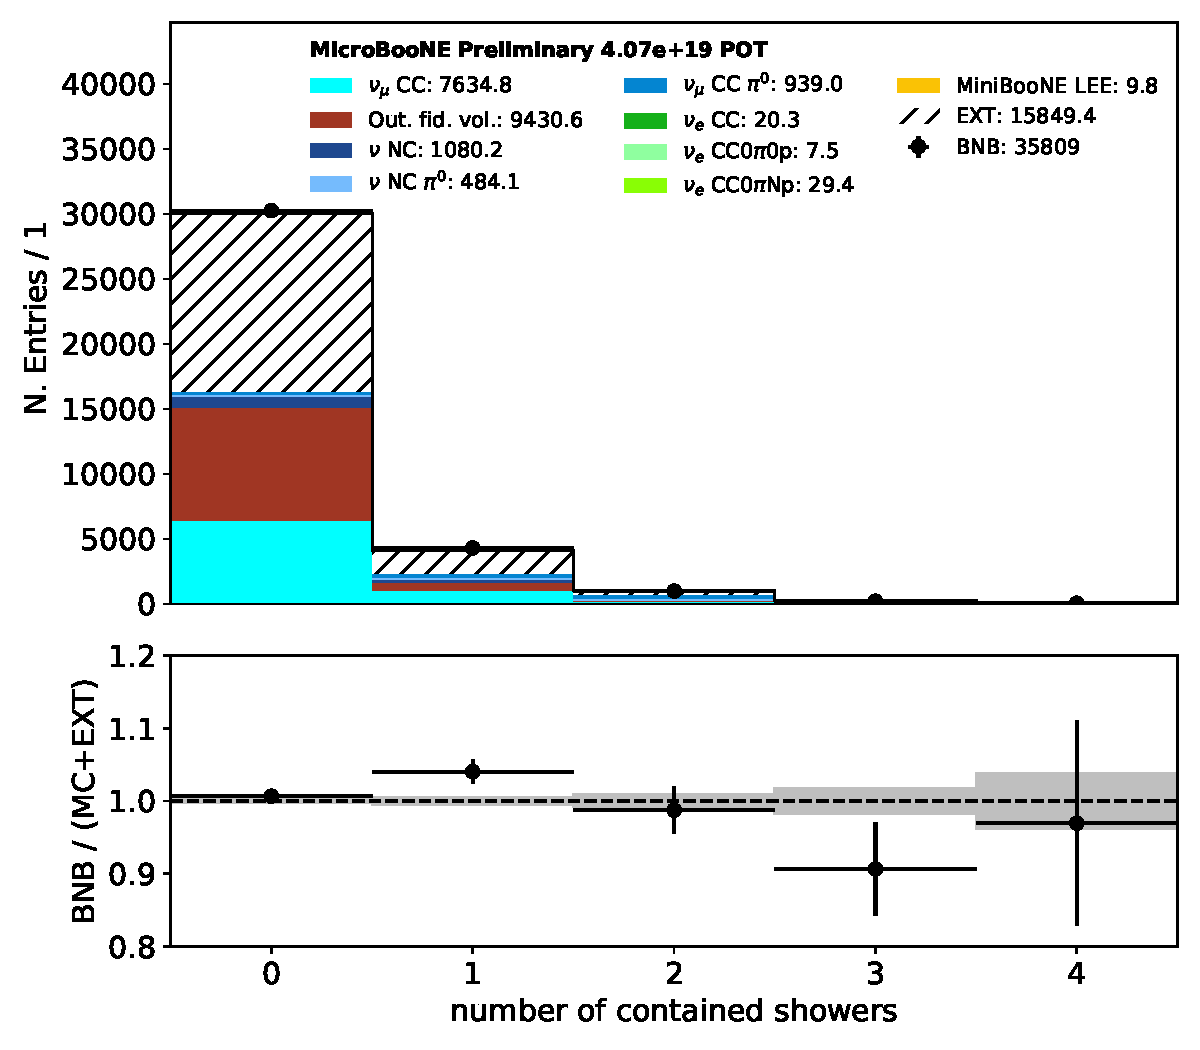
\includegraphics[width=1.00\textwidth]{nueselection/n_showers_contained_01132020_RUN1.pdf}
    \caption{\label{fig:nue:presel:nshower} }
    \end{subfigure}
    \begin{subfigure}[b]{0.3\textwidth}
    \centering
    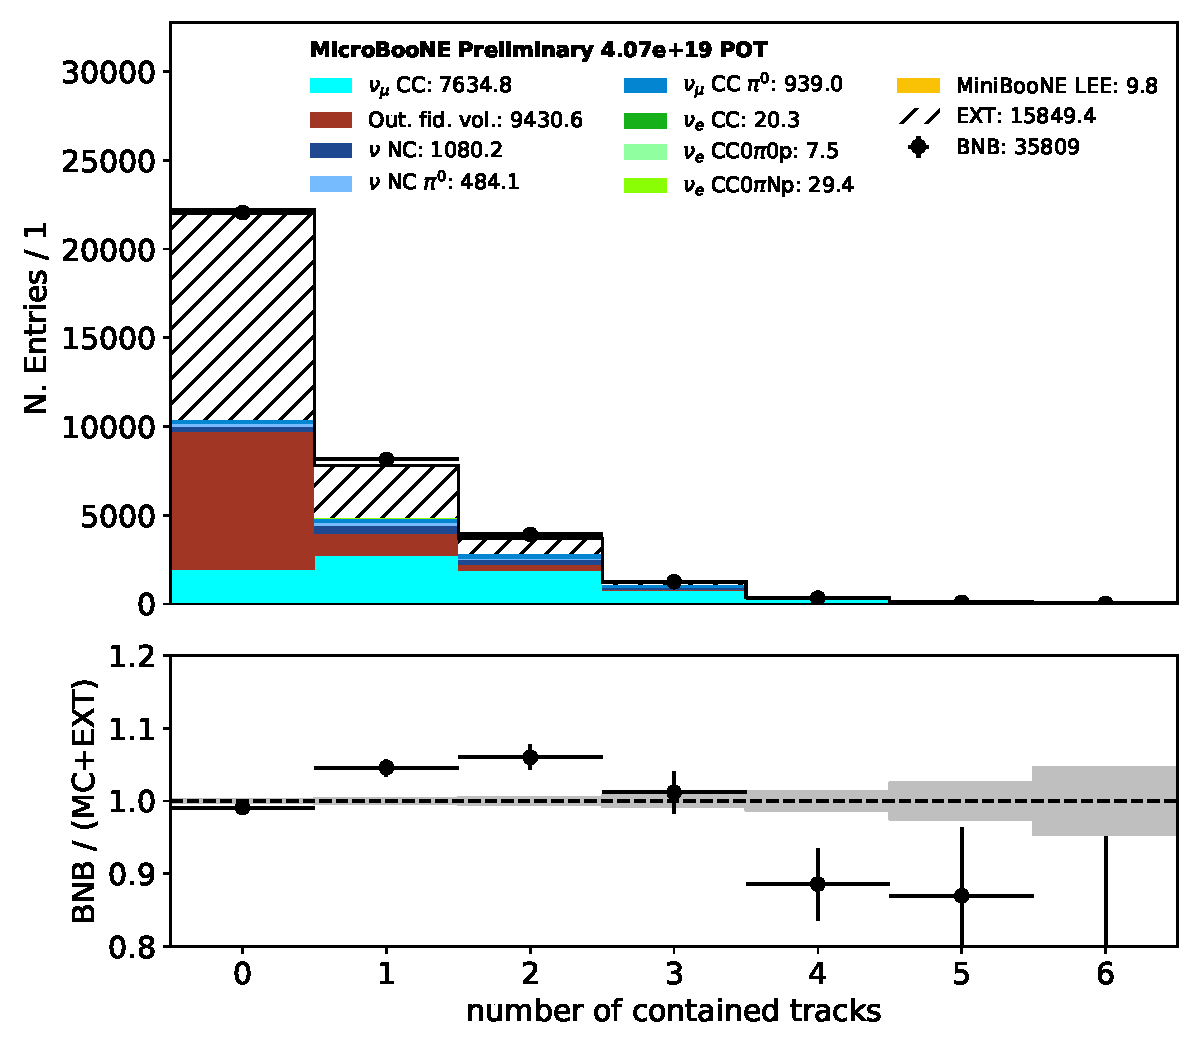
\includegraphics[width=1.00\textwidth]{nueselection/n_tracks_contained_01132020_RUN1.pdf}
    \caption{\label{fig:nue:presel:ntrack} }
    \end{subfigure}
    \begin{subfigure}[b]{0.3\textwidth}
    \centering
    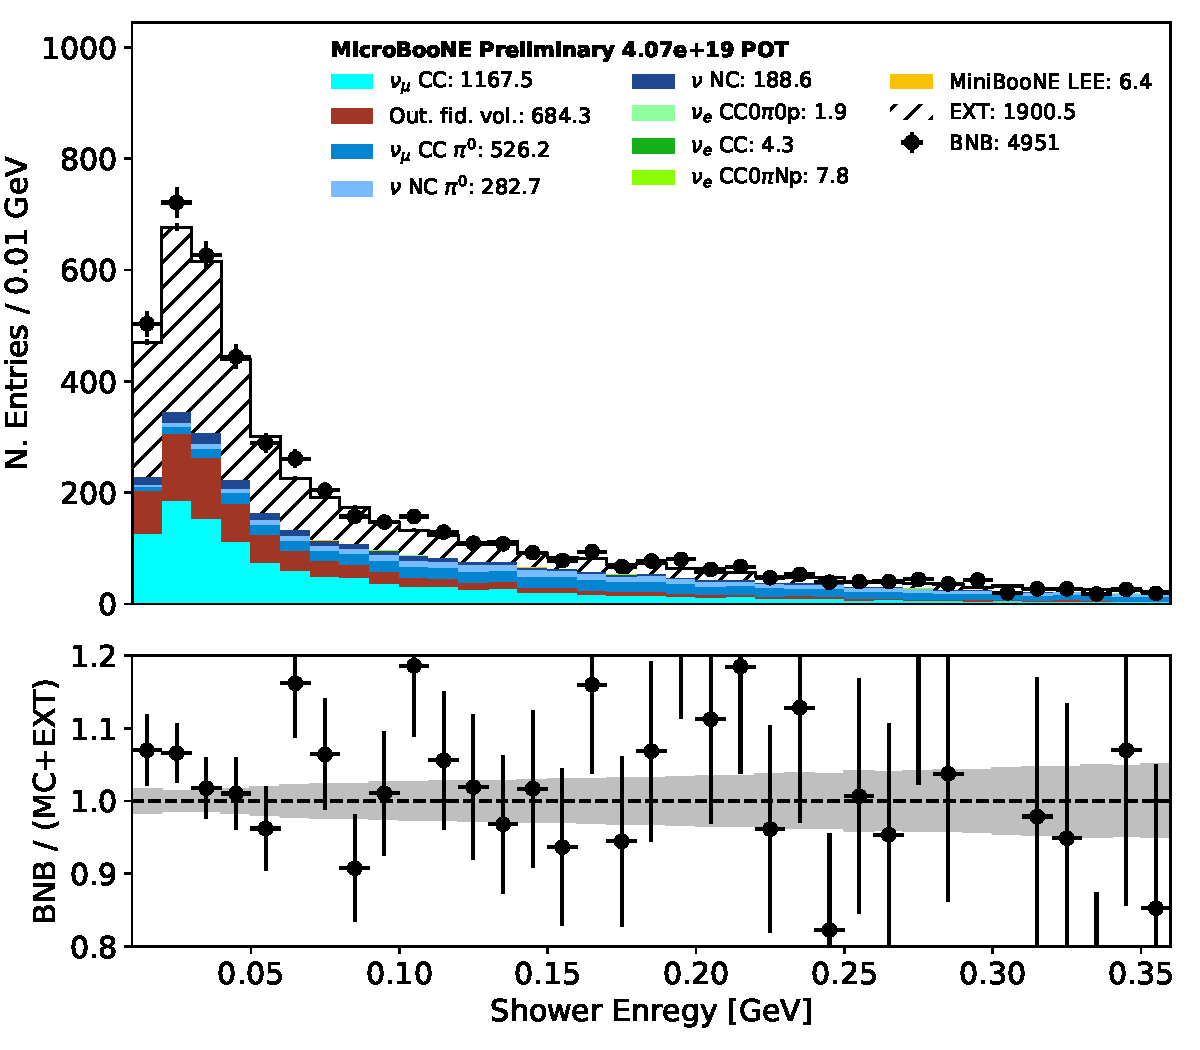
\includegraphics[width=1.00\textwidth]{nueselection/shr_energy_tot_cali_01132020_RUN1.pdf}
    \caption{\label{fig:nue:presel:shrenergy} }
    \end{subfigure}
\caption{\label{fig:nue:presel}Variables input to the common $\nu_e$ N$p$ and 0$p$ pre-selections.}
\end{center}
\end{figure}

\par The efficiencies of the 1$e$N$p$ and 1$e$0$p$ pre-selections are shown in figure~\ref{fig:nue:presel:eff}. Efficiencies are presented as a function of true neutrino energy~\ref{fig:nue:presel:eff:nu}, proton KE~\ref{fig:nue:presel:eff:proton}, and electron energy~\ref{fig:nue:presel:eff:elec}. Each plot shows in black the efficiency for the common pre-selection (before a proton requirement is or is not imposed) and is reported relative to all intrinsic $\nu_e$ events. In blue and red respectively are shown the efficiencies for the  1$e$N$p$ and 1$e$0$p$ selections respectively, for true N$p$ and 0$p$ events. Shaded histograms in red and blue show the stacked truth-level distributions for N$p$ and 0$p$ events for the variables being plotted.

\begin{figure}[H] 
\begin{center}
    \begin{subfigure}[b]{0.3\textwidth}
    \centering
    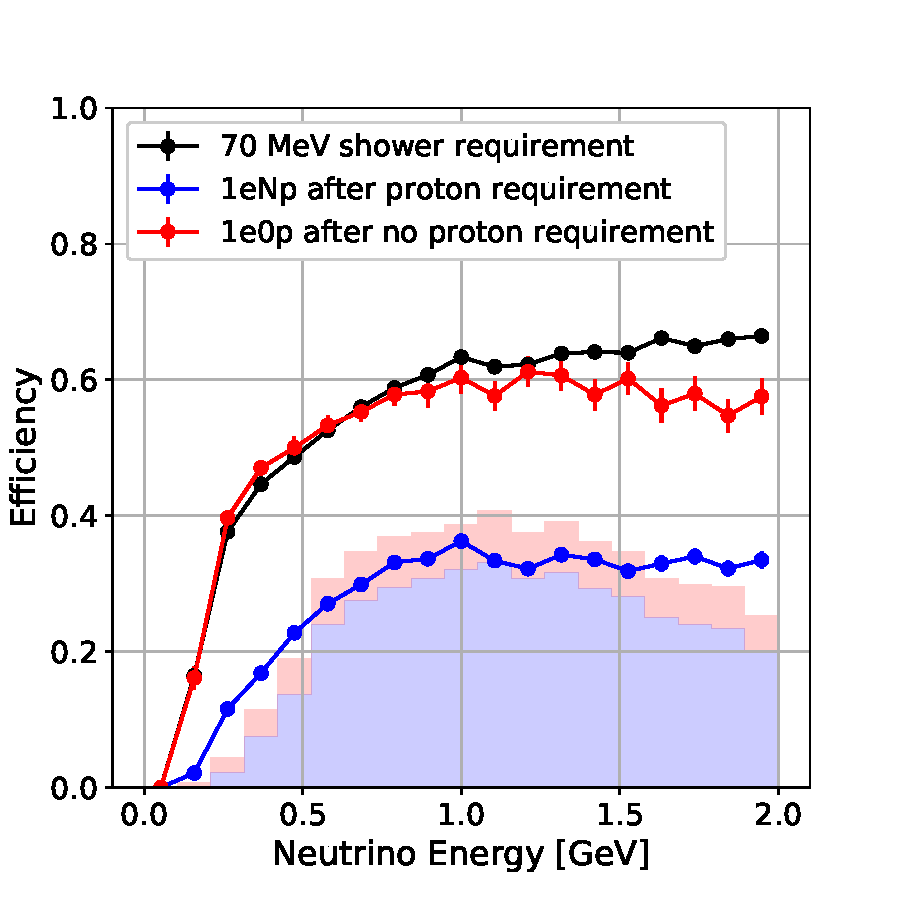
\includegraphics[width=1.00\textwidth]{nueselection/nu_RUN1.pdf}
    \caption{\label{fig:nue:presel:eff:nu} }
    \end{subfigure}
    \begin{subfigure}[b]{0.3\textwidth}
    \centering
    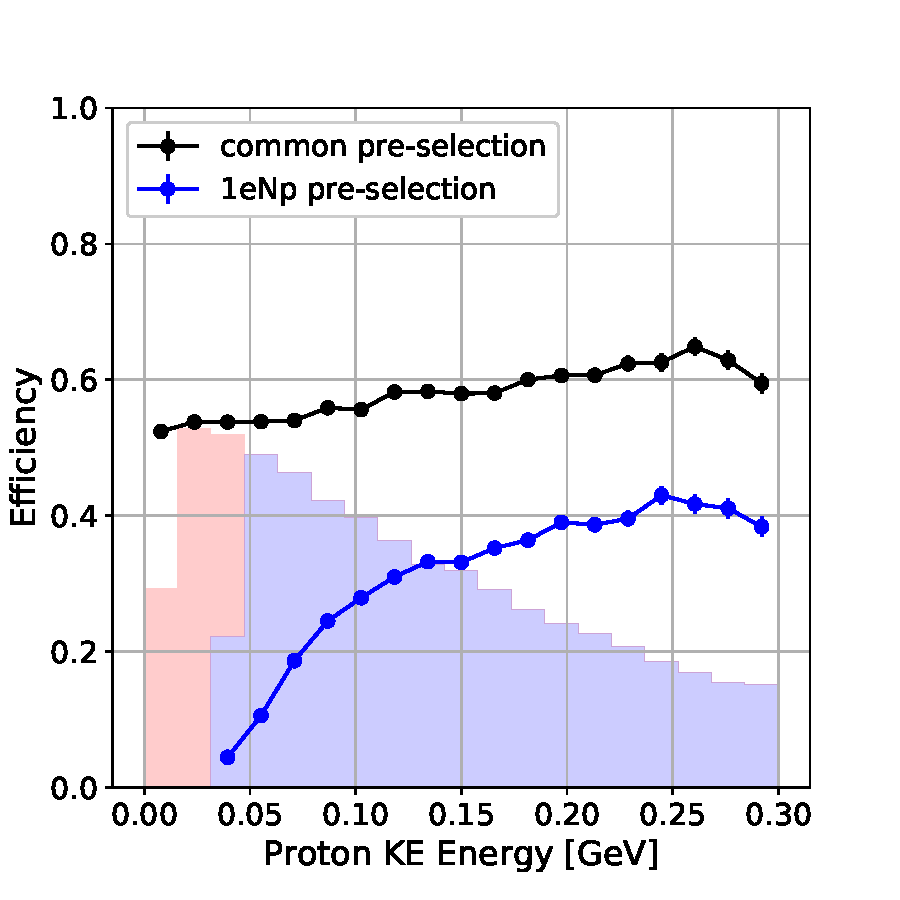
\includegraphics[width=1.00\textwidth]{nueselection/proton_RUN1.pdf}
    \caption{\label{fig:nue:presel:eff:proton} }
    \end{subfigure}
    \begin{subfigure}[b]{0.3\textwidth}
    \centering
    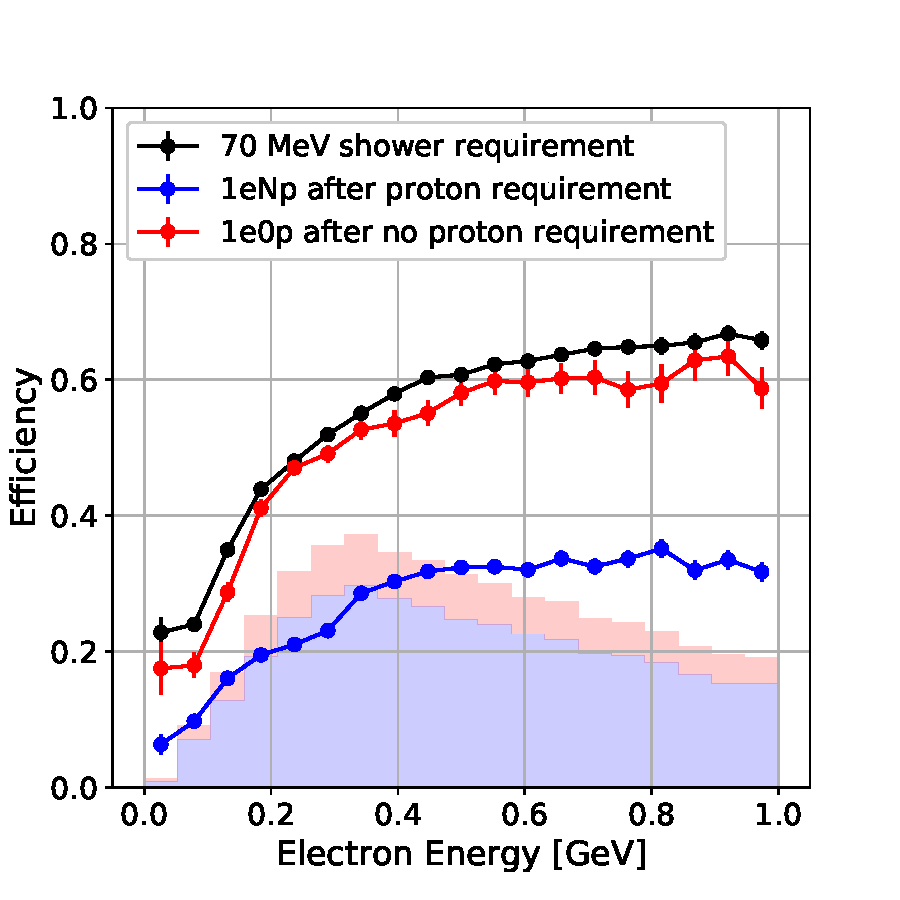
\includegraphics[width=1.00\textwidth]{nueselection/elec_RUN1.pdf}
    \caption{\label{fig:nue:presel:eff:elec} }
    \end{subfigure}
\caption{\label{fig:nue:presel:eff}}
\end{center}
\end{figure}

\subsection{Variable definitions}

\par \noindent  \textbf{Slice variables}:

\begin{itemize}
    \item \emph{nslice}: number of neutrino slices identified by the SliceId (possible values are 0 and 1);
    \item \emph{reco\_nu\_vtx\_sce\_\{x,y,z\}}: Reconstructed space charged corrected neutrino interaction vertex in (x,y,z) coordinates.
    \item \emph{n\_showers\_contained}: number of showers with a starting point within the fiducial volume;
    \item \emph{n\_tracks\_contained}: number of tracks fully contained in the fiducial volume;
    \item \emph{contained\_fraction}: fraction of hits in PFParticles contained in the fiducial volume (according to definitions above) with respect to the total number of clustered hits in the slice;
    \item \emph{hits\_ratio}: ratio between hits from showers and total number of hits;
    \item \emph{CosmicIP}: closest distance between shower start and space points associated to tracks flagged as cosmics.
    \item \emph{crtveto}
    \item \emph{\_closestNuCosmicDist}
\end{itemize}

\par \noindent \textbf{Shower and Track variables}:

\begin{itemize}
    \item \emph{tksh\_distance}: distance between leading shower vertex and longest track vertex;
    \item \emph{tksh\_angle}: angle between leading shower vertex and longest track vertex;
    item \emph{merge\_bestdist}: Distance between shower start point and track start (or end) point for the track in the slice that best matches the direction of the shower. 
\end{itemize}

\par \noindent \textbf{Shower variables}:

\begin{itemize}
    \item \emph{shr\_energy\_tot\_cali}: sum of the energy of the calibrated showers (in GeV);
    \item \emph{shr\_tkfit\_2cm\_dedx\_\{U,V,Y\}}: dE/dx in the first 2 cm of the leading shower on plane (U,V,Y) with the track fitting;
    \item \emph{shr\_tkfit\_gap10\_dedx\_\{U,V,Y\}}: dE/dx in the [1,5] cm range of the leading shower on plane (U,V,Y) with the track fitting;
    \item \emph{shr\_score}: Pandora SVM track/shower score for the leading shower;
    \item \emph{shrmoliereavg}: xxx
    \item \emph{subcluster}: number of subclusters (counted in all planes) for the leading shower.
    \item \emph{trkfit}: ratio of hits fitted in the track fit to the shower to all hits in the shower.
\end{itemize}

\par \noindent  \textbf{Track variables}:

\begin{itemize}
    \item \emph{trkpid}: proton-muon LLR particle identification 
\end{itemize}

\par \noindent  \textbf{$\pi^0$ rejection variables}:

\begin{itemize}
    \item \emph{secondshower\_Y\_nhit}:
    \item \emph{secondshower\_Y\_dot}:
    \item \emph{anglediff\_Y}:
    \item \emph{secondshower\_Y\_vtxdist}:
\end{itemize}

\subsection{Inclusive Channel}

\subsection{1$e$N$p$ Channel \textcolor{red}{David + Giuseppe}}

The 1$e$N$p$ channel is the most sensitive to the MiniBooNE eLEE signal as it contains a large fraction of the signal events and allows for selection requirements based both on showers and tracks. 
Given the large cosmic background and that $\nu_e$ charge-current interactions are O(1\%) in the BNB, a high-purity selection is needed to achieve a sizeable signal sensitivity. 

We first define a set of minimal requirements ("preselection") to obtain a high statistics sample (dominated by cosmic and neutrino backgrounds) that is used to monitor the data-MC agreement of the selection variables. 
We then define two alternative selections, respectively based on a simple box-cut approach and on boosted decision trees (BDT); the BDT approach is clearly the most sensitive, while box-cuts provide a robust reference selection.

\par \textbf{Preselection}:

At preselection stage we apply the minimum set of requirements so that all selection variabes can be defined, plus the containment and a minimum shower energy to reject Michel electrons:
\begin{itemize}
    \item nslice = 1
    \item n\_tracks\_contained $>$ 0
    \item n\_showers\_contained $>$ 0
    \item contained\_fraction $>$ 0.9
    \item shr\_energy\_tot\_cali $>$ 0.07
\end{itemize}

\par 
Topics to discuss: selection efficiency and purity, data-MC agreement of selection variables.

\begin{figure}[ht] 
\begin{center}
    \begin{subfigure}[b]{0.45\textwidth}
    \centering
    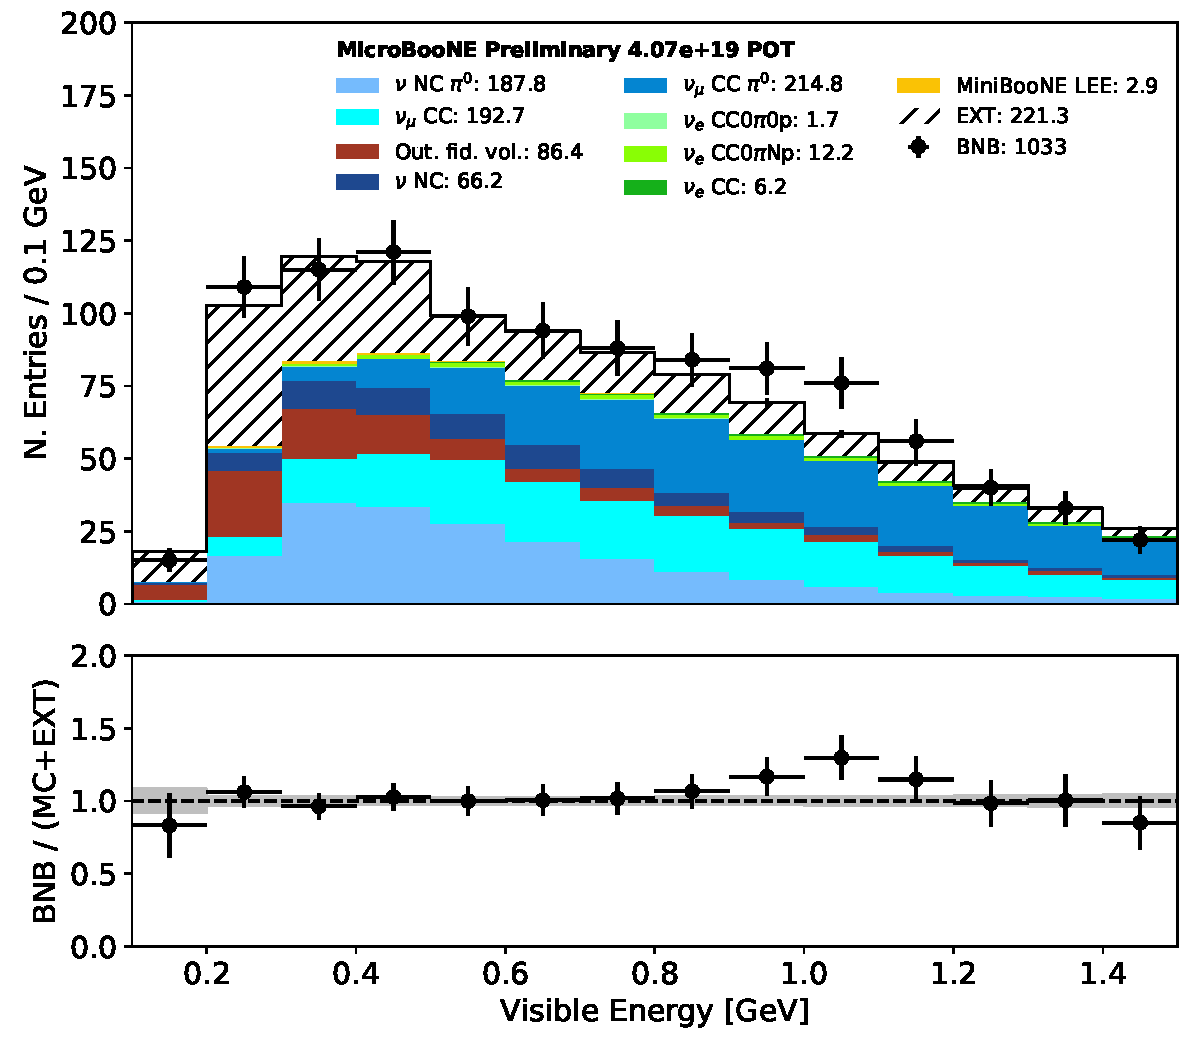
\includegraphics[width=1.00\textwidth]{1eNp/reco_e_01122020_RUN1.pdf}
    \caption{\label{fig:1eNp:prsel:RUN1} RUN 1}
    \end{subfigure}
    \begin{subfigure}[b]{0.45\textwidth}
    \centering
    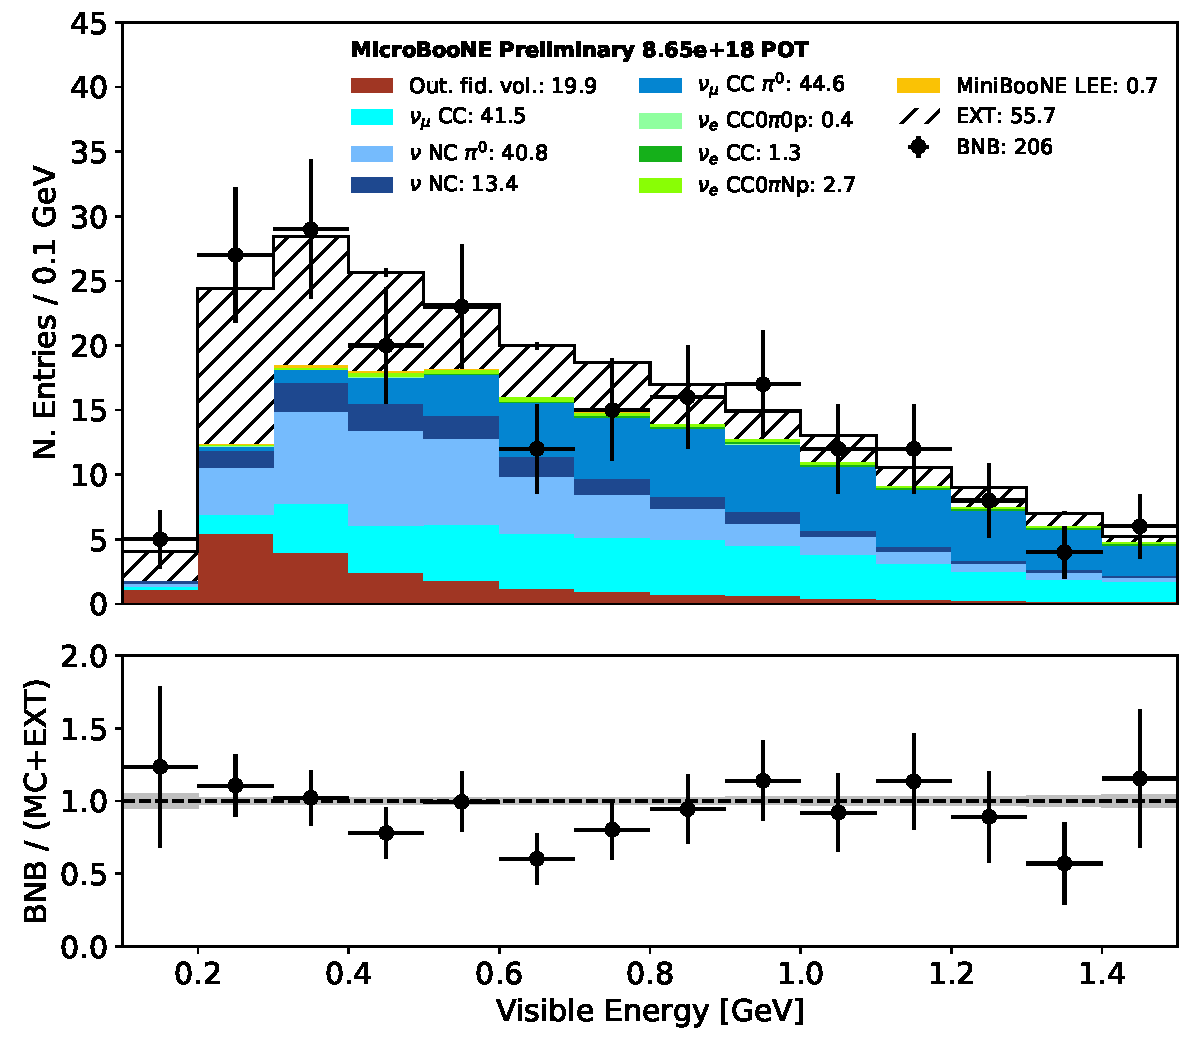
\includegraphics[width=1.00\textwidth]{1eNp/reco_e_01122020_RUN3.pdf}
    \caption{\label{fig:1eNp:prsel:RUN1} RUN 3}
    \end{subfigure}
\caption{\label{fig:1eNp:prsel}pre-selection for 1$e$N$p$ channel}
\end{center}
\end{figure}

\par \textbf{Box-cuts}:

In addition to the preselection requirements, cuts are applied to suppress specific backgrounds.
Cosmics are rejected by requiring large CosmicIP and a proton-like trkpid.
Events from $\nu_\mu$ charged current interactions are suppressed requiring shower hits to be the dominant in the slice, and imposing tight quality requirements on the shower object (shr\_score, shrmoliereavg, trkfit, subcluster).
Events with $\pi^0$ are rejected requiring only one shower in the event, a small distance between the track and shower start points, that the shower dEdx can be evaluated at least on the collection plane and it is not consistent with two or more MIPs in any plane (using two different dEdx definitions).
Finally, in order to avoid misreconstructed events, events where the track and shower are aligned are rejected.

The full list of cuts is:
\begin{itemize}
    \item CosmicIP $>$ 20.
    \item trkpid $<$ -0.02
    \item hits\_ratio $>$ 0.60
    \item shr\_score $<$ 0.275
    \item shrmoliereavg $>$ 2 and shrmoliereavg $<$ 9
    \item trkfit $<$ 0.45 or subcluster $>$ 6
    \item n\_showers\_contained = 1
    \item tksh\_distance $<$ 3.5
    \item shr\_tkfit\_2cm\_dedx\_Y $\in$ [0,4.0] and shr\_tkfit\_2cm\_dedx\_U $<$ 4.0 and shr\_tkfit\_2cm\_dedx\_V $<$ 4.0
    \item shr\_tkfit\_gap10\_dedx\_Y $\in$ [0,4.5] and shr\_tkfit\_gap10\_dedx\_U $<$ 4.5 and shr\_tkfit\_gap10\_dedx\_V $<$ 4.5
    \item secondshower\_Y\_nhit $\leq$ 8 or secondshower\_Y\_dot $\leq$ 0.8 or anglediff\_Y $\leq$ 40 or secondshower\_Y\_vtxdist $\geq$ 100
    \item tksh\_angle $>$ -0.9 and tksh\_angle $<$ 0.7
\end{itemize}

\par 
Topics to discuss: selection efficiency and purity, expected number of events in open data and in full sample.

\begin{figure}[ht]
\begin{center}
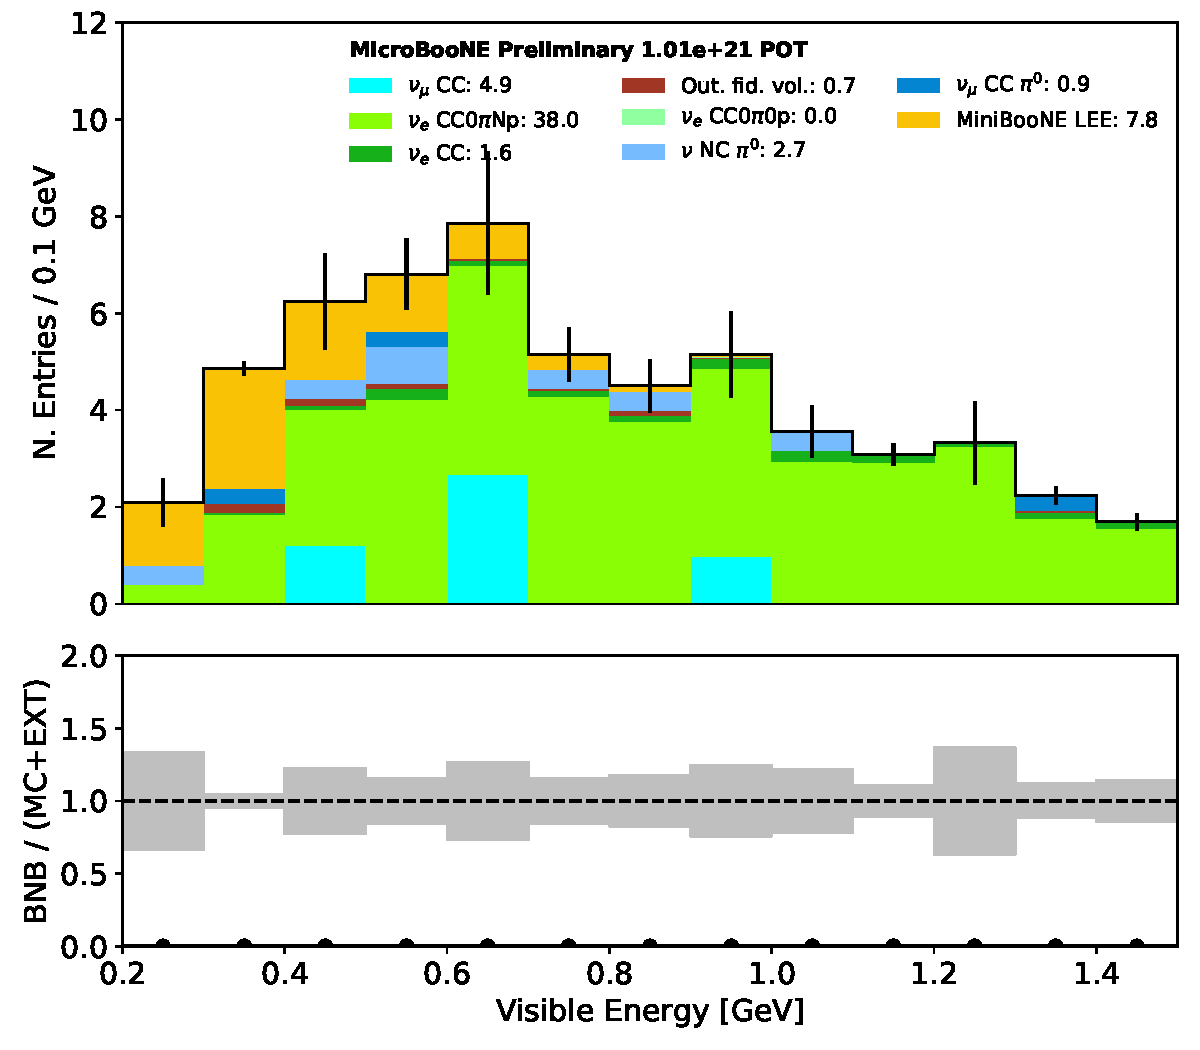
\includegraphics[width=0.45\textwidth]{1eNp/reco_e_01122020_RUN1_box.pdf}
\caption{\label{fig:1eNp:box:RUN1}Box-cuts for 1$e$N$p$ channel.}
\end{center}
\end{figure}

\par \textbf{BDT}:

Two BDTs are trained separately to reject backgrounds with and without $\pi^0$ in the final state. The same set of training variables is used in the two BDTs, corresponding to the list of variables used in the box-cut selection. 

Both in the training and in the analysis, events are required to pass the preselection requirements plus a loose set of cuts intended to avoid considering events where one or more variables is clearly inconsistent with $\nu_e$ events. The list of cuts is:
\begin{itemize}
    \item CosmicIP $>$ 20.
    \item trkpid $<$ 0.1
    \item hits\_ratio $>$ 0.5
    \item shr\_score $<$ 0.30
    \item n\_showers\_contained = 1
    \item tksh\_distance $<$ 6.0
    \item shr\_tkfit\_2cm\_dedx\_Y $<$ 4.0
    \item tksh\_angle $>$ -0.9
\end{itemize}

Indeed the BDT is able to figure out during training which variables are most important for each background: shower quality variables (e.g. shr\_score, trkfit, subcluster) have higher ranking for the non-$\pi^0$ BDT, while variables such as tksh\_distance and the shower dEdx show higher importance for the $\pi^0$-BDT. It is interesting to note that the most discriminating variable is in both cases shrmoliereavg which may be useful to discriminate both muons in $\nu_\mu$ events (low values) and merged showers in $\pi^0$ events (large values).

\begin{table}[h!]
\centering
 \begin{tabular}{c | c c | c c} 
 \hline
& \multicolumn{2}{c |}{$\pi^0$ BDT} & \multicolumn{2}{c}{non-$\pi^0$ BDT} \\
 \hline
Rank & Variable & Importance & Variable & Importance \\
 \hline
1 & shrmoliereavg & 5813 & shrmoliereavg & 6436 \\ 
2 & tksh\_distance & 2834 & trkfit & 3309 \\
3 & trkpid & 2306 & shr\_tkfit\_2cm\_dedx\_ALL & 1980 \\
4 & shr\_tkfit\_2cm\_dedx\_ALL & 2225 & subcluster & 1908 \\
5 & secondshower\_Y\_vtxdist & 1891 & shr\_score & 1851 \\
6 & shr\_tkfit\_gap10\_dedx\_ALL & 1702 & trkpid & 1778 \\
7 & shr\_score & 1572 & secondshower\_Y\_vtxdist & 1405 \\
8 & trkshrhitdist2 & 1286 & shr\_tkfit\_gap10\_dedx\_ALL & 1293 \\
9 & trkfit & 1101 & tksh\_distance & 981 \\
10 & secondshower\_Y\_nhit & 1015 & secondshower\_Y\_nhit & 976 \\
11 & hits\_ratio & 949 & anglediff\_Y & 914 \\
12 & tksh\_angle & 929 & trkshrhitdist2 & 903 \\
13 & anglediff\_Y & 831 & tksh\_angle & 881 \\
14 & subcluster & 699  & hits\_ratio & 657 \\
15 & secondshower\_Y\_dot & 680 & secondshower\_Y\_dot & 592 \\
 \hline
\end{tabular}
\caption{Ranking of BDT variables based on their importance in terms of "total gain". dEdx variables are combined for different planes (note the "ALL" suffix).}
\label{tab:bdtimp}
\end{table}

We then cut separately on the output of the two BDTs, requiring pi0\_score $>$ 0.995 and nonpi0\_score $>$ 0.9984.

\par 
Topics to discuss: selection efficiency and purity, expected number of events in open data and in full sample.

\begin{figure}[H] 
\begin{center}
    \begin{subfigure}[b]{0.45\textwidth}
    \centering
    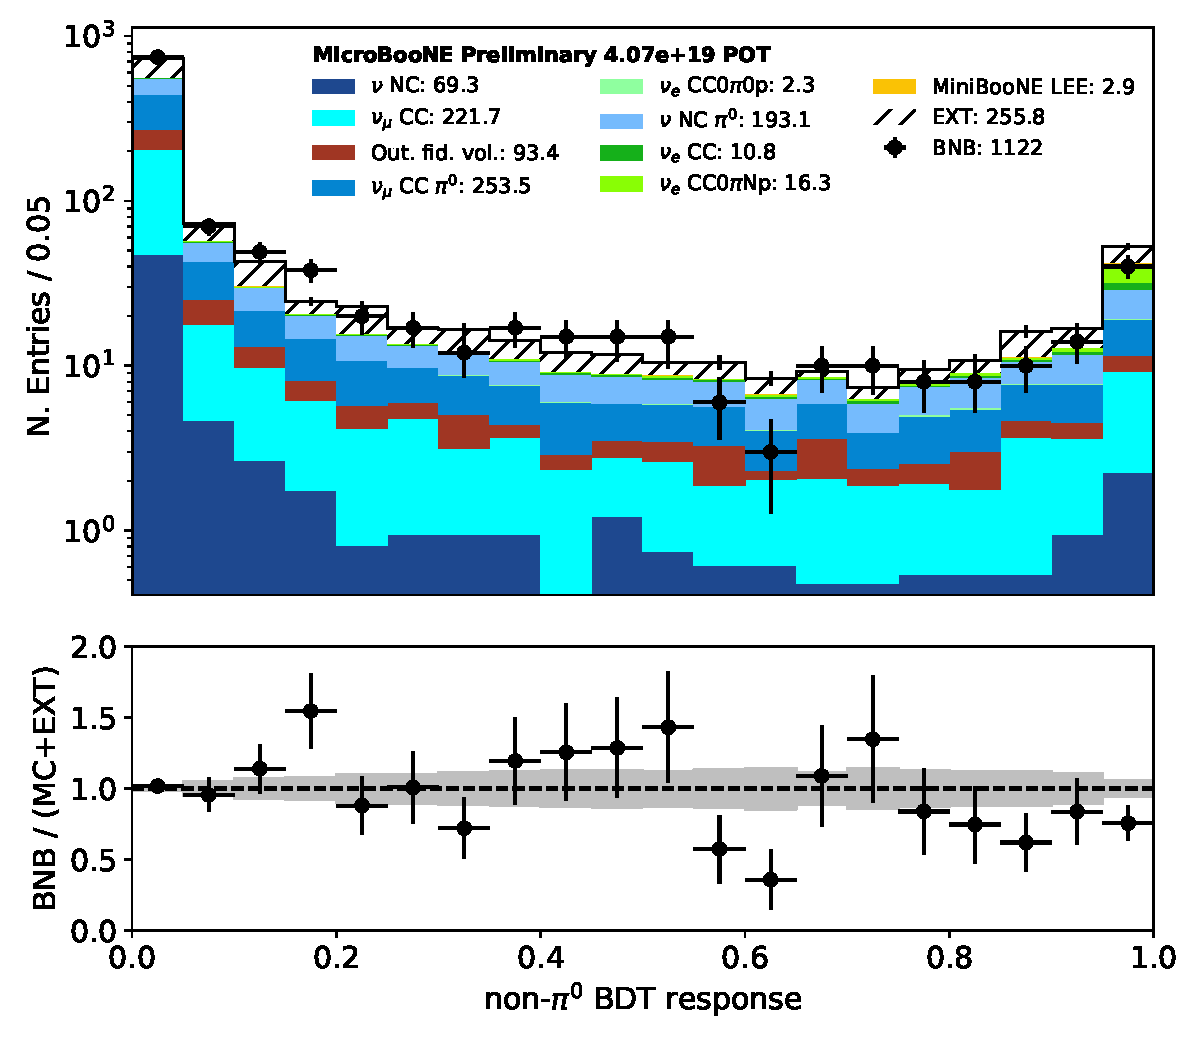
\includegraphics[width=1.00\textwidth]{1eNp/nonpi0_score_01122020_RUN1.pdf}
    \caption{\label{fig:1eNp:bdt:nonpi0:all}}
    \end{subfigure}
    \begin{subfigure}[b]{0.45\textwidth}
    \centering
    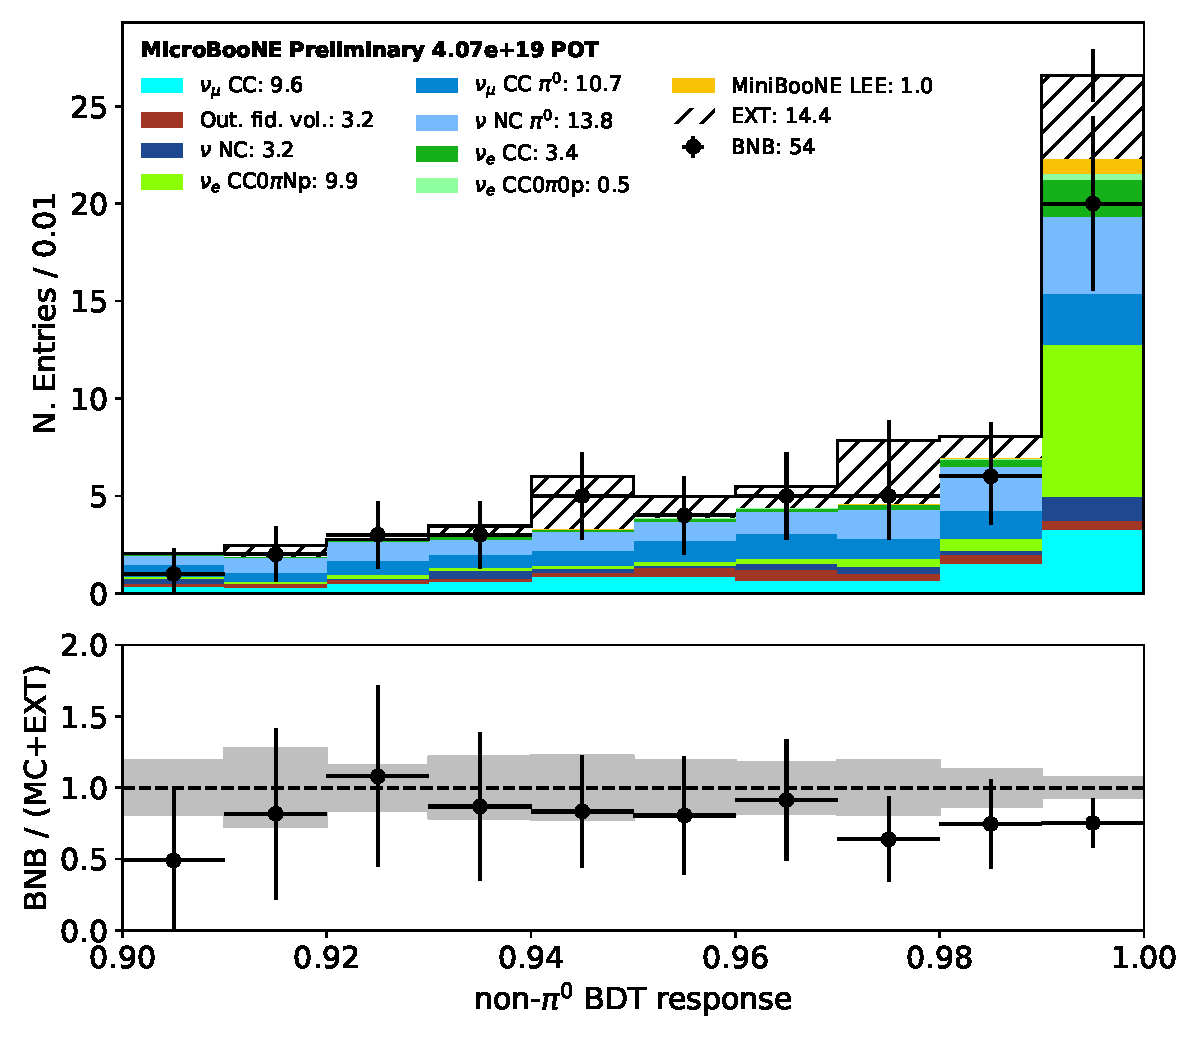
\includegraphics[width=1.00\textwidth]{1eNp/nonpi0_score_01122020_zoom_RUN1.pdf}
    \caption{\label{fig:1eNp:bdt:nonpi0:zoom}}
    \end{subfigure}
\caption{\label{ffig:1eNp:bdt:nonpi0}BDT resposne for non-$\pi^0$ BDT after 1$e$N$p$ pre-selection}
\end{center}
\end{figure}


\begin{figure}[H] 
\begin{center}
    \begin{subfigure}[b]{0.45\textwidth}
    \centering
    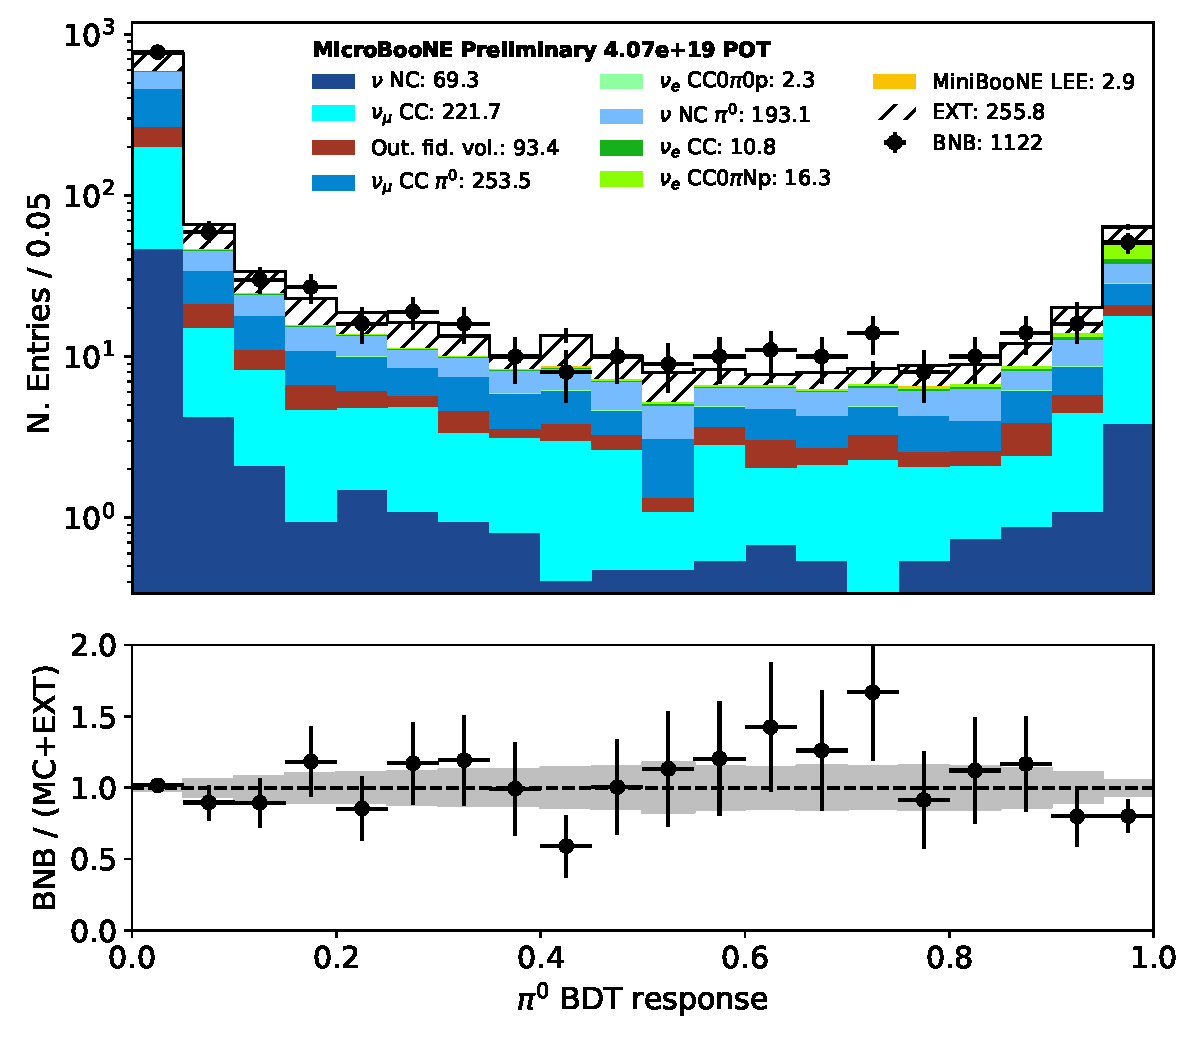
\includegraphics[width=1.00\textwidth]{1eNp/pi0_score_01122020_RUN1.pdf}
    \caption{\label{fig:1eNp:bdt:pi0:all}}
    \end{subfigure}
    \begin{subfigure}[b]{0.45\textwidth}
    \centering
    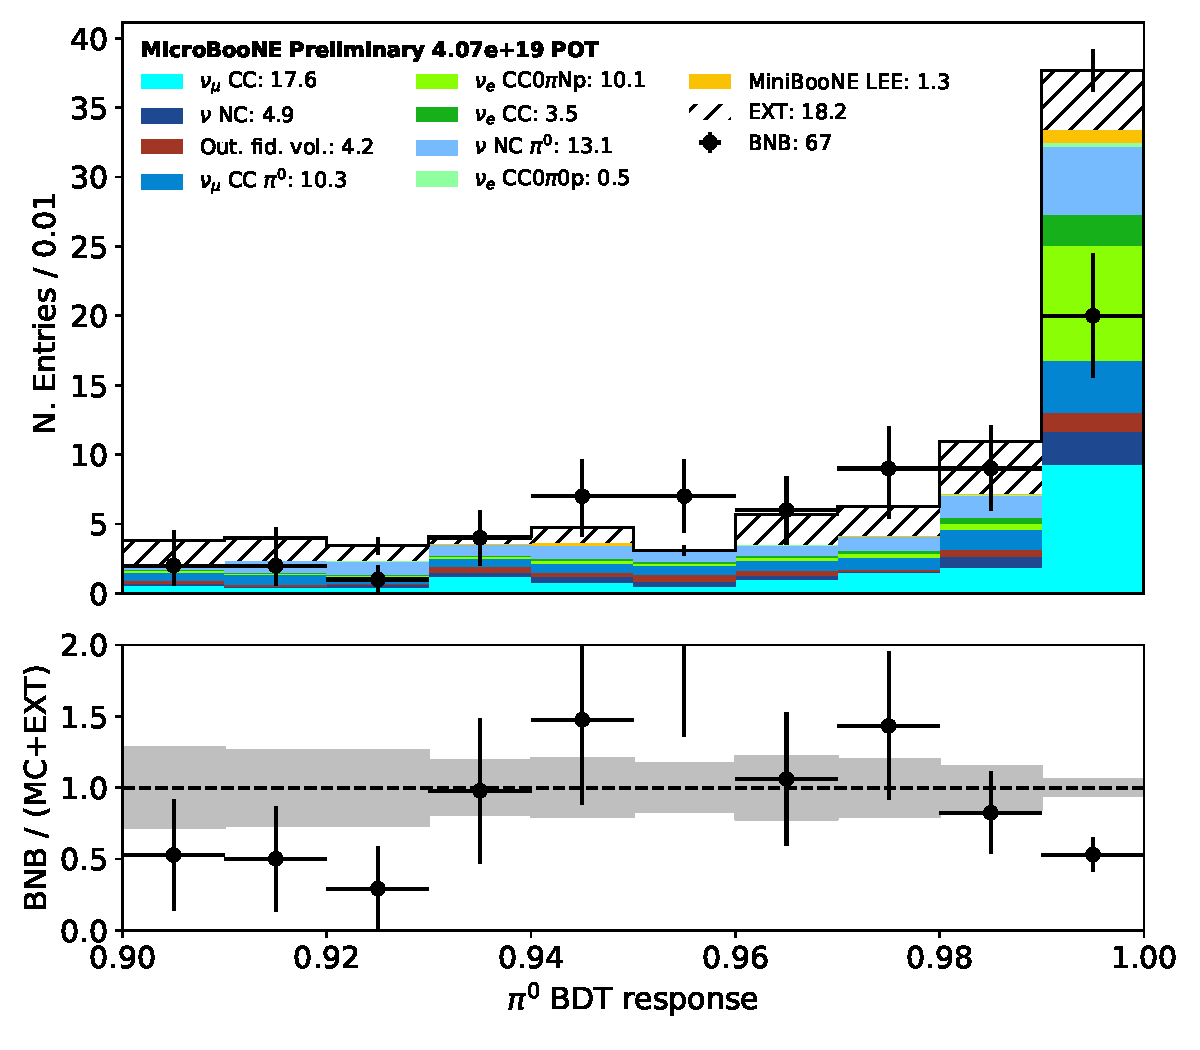
\includegraphics[width=1.00\textwidth]{1eNp/pi0_score_01122020_zoom_RUN1.pdf}
    \caption{\label{fig:1eNp:bdt:pi0:zoom}}
    \end{subfigure}
\caption{\label{ffig:1eNp:bdt:pi0}BDT resposne for $\pi^0$ BDT after 1$e$N$p$ pre-selection}
\end{center}
\end{figure}

\begin{figure}[H]
\begin{center}
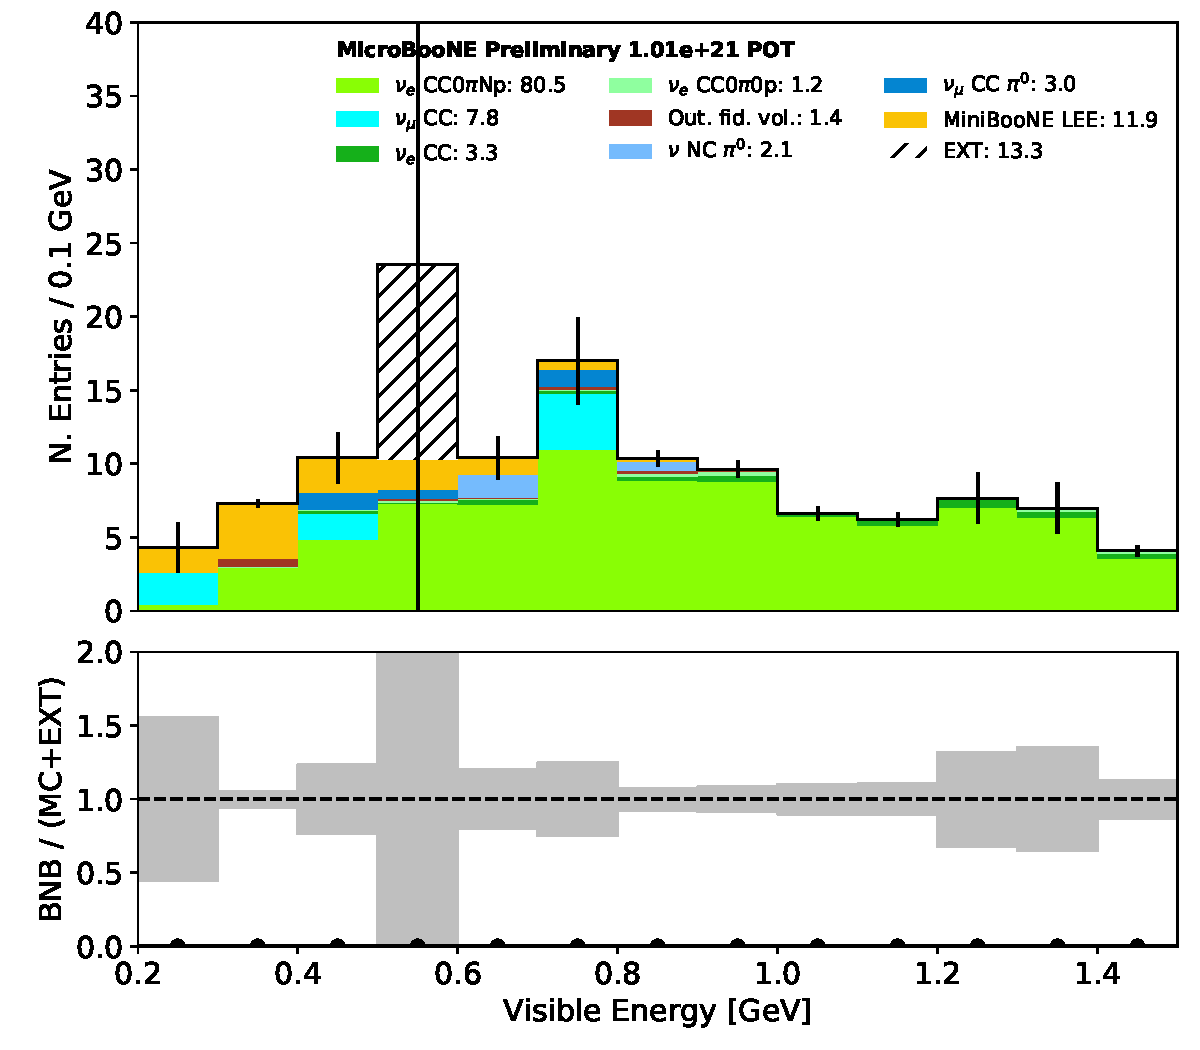
\includegraphics[width=0.45\textwidth]{1eNp/reco_e_01122020_bdt_RUN1.pdf}
\caption{\label{fig:1eNp:box:RUN1}BDT-based selection for 1$e$N$p$ with cuts at 0.995 and 0.9984 for the $\pi^0$ and non-$\pi^0$ variables respectively.}
\end{center}
\end{figure}


\subsection{1$e$0$p$ Channel \textcolor{red}{Sophie, Ivan}}
Selection motivation:

\subsubsection{Tools Unique to 0p Selection}
Shower-Track merging to recover signal orthogonal to Np selection.

\subsubsection{Pre-selection}
Data-MC comparisons:

\subsubsection{Box cut selection}

\subsubsection{BDT}

\newpage
\section{$\nu_{\mu}$ Selection}

\newpage

\section{Systematics \textcolor{red}{Maya, Nicolo, Sebastien}}
\label{sec:systematics}
\subsection{Detector Systematics}
The details on detector systematics can be found in~\cite{bib:detsyssupportnote}. To asses the detector systematics uncertainties in the eLEE analysis, the following detector variations samples are used:
\begin{enumerate}
    \item Uncorrelated unisims for waveform variations in examined variables ($x$, $y$, $z$, $\theta_{XZ}$, $\theta_{YZ}$, $dE/dx$), where the waveform variations as function of $dE/dx$ may be replaced by dedicated recombination unisim.
    \item Unisim for light yield simulation uncertainty.
    \item Unisim for Space Charge Effects uncertainty.
\end{enumerate}

\subsection{Flux Uncertainties}
The flux and uncertainties for MCC9~\cite{bib:fluxmcc9} are largely the same as MCC8~\cite{bib:fluxtechnote}.  
\subsection{Neutrino Interaction Modeling Uncertainties}
Document~\cite{bib:geniesupportnote} describes the GENIE cross-section model, recommended central-value tune, and the recommended uncertainties for MCC9 analyses. 

\newpage

\section{Sensitivity Estimation ID \textcolor{red}{Nico + ...}}
\label{sec:sensitivity}
\par This document is primarily focused on presenting sensitivities for a specific signal hypothesis:  
\subsection{Test Statistics and Statistics-Only Sensitivities}
The test statistics are performed through the SBNfit tool~\cite{bib:sbnfit20437} and a separate stand-alone tool that is primarily used to crosscheck and understand SBNfit. The stand-alone test statistics tool is also used for performing additional test statistics not covered by the SBNfit, such as the Poisson log likelihood  ratio test statistics.
\subsection{How Constraints and Systematics are included in the 1$e$N$p$ Sensitivity Calculation}

\subsubsection{Constraint from Muon Neutrino}
\subsection{Final Sensitivities}

\newpage
\section{Conclusions and Outlook}

\newpage


\appendix

\section{Data-MC Comparisons}

\section{Code Repositories}

\begin{thebibliography}{}
\bibitem{bib:pandoraub} 
  R.~Acciarri {\it et al.} [MicroBooNE Collaboration],
  \emph{The Pandora multi-algorithm approach to automated pattern recognition of cosmic-ray muon and neutrino events in the MicroBooNE detector}, Eur.\ Phys.\ J.\ C {\bf 78}, no. 1, 82 (2018) [arXiv:1708.03135 [hep-ex]].
\bibitem{bib:tkshsvm}
L. Escudero Sanchez, \emph{Updates on SVM-based track/shower identification in Pandora},
\href{https://microboone-docdb.fnal.gov/cgi-bin/private/ShowDocument?docid=14039}{DocDB 14039}
\bibitem{bib:pi0reco}
  C.~Adams {\it et al.} [MicroBooNE Collaboration],
  \emph{Reconstruction and Measurement of $\mathcal{O}$(100) MeV Energy Electromagnetic Activity from $\pi^0 \rightarrow \gamma\gamma$ Decays in the MicroBooNE LArTPC},  arXiv:1910.02166 [hep-ex].
\bibitem{bib:shrtrackfitter}
G. Cerati, \emph{Track fits to main shower trunk and improved dEdx}, \href{https://microboone-docdb.fnal.gov/cgi-bin/private/ShowDocument?docid=20824}{DocDB 20824}
\bibitem{bib:detsyssupportnote}
A. Ashkenazi, et al., \emph{Detector Systematics supporting note}, \href{https://microboone-docdb.fnal.gov/cgi-bin/private/ShowDocument?docid=27009}{DocDB 27009}
\bibitem{bib:fluxmcc9}
Z. Pavlović, \emph{BNB Flux}, \href{https://microboone-docdb.fnal.gov/cgi-bin/private/RetrieveFile?docid=26985}{DocDB 26985}
\bibitem{bib:fluxtechnote}
Z. Pavlović, \emph{Booster Neutrino Flux Prediction at MicroBooNE}, \href{https://microboone-docdb.fnal.gov/cgi-bin/private/RetrieveFile?docid=15444}{DocDB 15444}
\bibitem{bib:geniesupportnote}
K. Duffy, et al., \emph{Supporting note: Cross-section model and uncertainties}, \href{https://microboone-docdb.fnal.gov/cgi-bin/private/ShowDocument?docid=27018}{DocDB 27018}
\bibitem{bib:sbnfit20437}
M. Ross-Lonergan, \emph{From MiniBooNE data to MicroBooNE LEE sensitivity: A step-by-step review and guide},\href{https://microboone-docdb.fnal.gov/cgi-bin/private/RetrieveFile?docid=20437}{DocDB 20437}
\bibitem{bib:CRTPresel_Technote}
D. Caratelli, et al., \emph{Use of the MicroBooNE Cosmic Ray Tagger for Electron Neutrino Preselection}, \href{https://microboone-docdb.fnal.gov/cgi-bin/private/RetrieveFile?docid=24031&filename=CRTPACTechnote.pdf&version=1}{DocDB 24031}

\end{thebibliography}

\end{document}


